% !TEX root = diss.tex

\chapter{Do non-redox active metal cations have the potentials to behave as
chemo-protective agents? The Effects on Metal Cations on HAT Reaction Barrier
Heights} \label{ch:hat}

\section{Introduction}

Metal cations are ubiquitous in biological systems and play an important role
in biological function. As such, there is a great deal of interest in studying
metals in biological systems. Proteins in particular are often associated with
metals, and in the worldwide Protein Data Bank,\cite{Harding2010, Berman2007}
over one-third of crystal structures contain metals. Redox active metals, such
as copper and iron, act as co-factors in metalloenzymes for important catalytic
processes.\cite{Atkins2010}

Non-redox active metal cations are equally as important in biological function
as redox active metals, where they are essential to protein structure and
function, along with cellular and neuronal signalling.\cite{Karp1999} Sodium
and calcium ions are most abundant extracellularly, while potassium and
magnesium are dominant inside of cells. While specific ionic concentrations
vary dramatically depending on physiological conditions, estimates for
equilibrium concentrations in both mammalian heart cells\cite{Ingwall2006} and
blood plasma\cite{daSilva2001} are listed in~\ref{tab:metalconc}. As sodium and
magnesium are most abundant alkali and alkaline earth metals found in
biologically relevant systems, they are of prime interest for investigation.

\begin{table}[!htbp]
  \caption{Ionic concentrations inside a mammalian heart cell and in the blood
  plasma. Concentrations are in units of mM. Values are rounded to one
  significant figure. Data are from Ref. \protect\citenum{Ingwall2006} and
  \protect\citenum{daSilva2001}.} \label{tab:metalconc}
\begin{tabular}{l c c}
  Ion Conc. & Mammalian Cells & Blood Plasma \\
  \hline
  \ch{Na^+} & 10 & 100--200 \\
  \ch{Mg^{2+}} & 10 & 1 \\
  \ch{K^+} & 100 & 4 \\
  \ch{Ca^{2+}} & 0.1 & 2
\end{tabular}
\end{table}

Extensive crystallographic surveys indicate that metals bind predominantly to
oxygen centres in proteins.\cite{Harding1999, Harding2004, Hsin2008} Divalent
metals are most often found bound directly to proteins. Calcium binds anywhere
from 4 to 6 binding sites in protein crystal structures, while magnesium binds
only 1 or 2. Monovalent metals, on the other hand, are often heavily solvated
and so they appear in solvent cavities of proteins, although sodium or
potassium are sometimes found bound directly to carbonyl or carboxylate oxygen
centres.\cite{Harding2010}

A great deal of research has focussed on \ch{Ca^{2+}} in the context of
reactive oxygen-centred radical production.\cite{Goerlach2015} Specifically,
\ch{Ca^{2+}} ions are important in the mitochondria, where, depending on
physiological conditions and concentrations, they can act as inhibitor or
promoters of free-radical production in the electron transport
chain.\cite{AdamVizi2010} One explanation is that \ch{Ca^{2+}} induce
conformational changes of the proteins involved in the electron transport chain
which are responsible for radical generation.\cite{Brookes2004} Mitochondrial
free-radicals, when present in moderate amounts, can act as cell signalling
molecules to activate pro-growth responses.\cite{Sullivan2014} However,
``dysfunctional'' mitochondria can produce excess radicals leading to oxidative
damage which has been linked to degenerative diseases.

Given the significant importance alkali and alkaline earth metals play in
biological systems, their impact on protein oxidation must be considered.
However, until recently, kinetic studies of protein oxidation have not
investigated the mechanistic role of non-redox active metals. In a series of
three papers,\cite{Salamone2013a, Salamone2015metals, Salamone2016} Bietti and
colleagues have shown that alkali and alkaline earth metals have an inhibitory
effect on HAT reactions involving \cumo\ and organic substrates. Some of the
experimental rate constants from these papers are summarized
in~\ref{tab:hat-metals}. All rate constants were obtained by time-resolved LFP
in nitrogen or argon-saturated acetonitrile (MeCN) at 298 K, as was previously
described in Section~\ref{sec:hat-methods}. The experimental results have been
rationalized on the basis of Lewis acidic metals cations interactions with
Lewis basic substrates.


\begin{table}
  \caption{Summary of rate constants for reactions of \cumo\ with various
  organic substrates in the presence of alkali and alkaline earth metal salts.}
  \label{tab:hat-metals}
  \hspace*{-1.2cm}
  \begin{tabular}{l l c c}
    Substrate & Conditions & $k_H$ (\Ms) & $k_H$(MeCN)/$k_H$(M$^{n+}$) \\
    \hline
    1,4-cyclohexadiene &    & 6.7\E{7} & \\
    (CHD)  & \ch{LiClO4} 1.0 M & 7.5\E{7} & 0.89 \\
     & \ch{Mg(ClO4)2} 1.0 M & 7.0\E{7} & 0.96 \\
    tetrahydrofuran &   & 5.7\E{6} & \\
    (THF) & \ch{LiClO4} 1.0 M & 2.9\E{6} & 1.7 \\
     & \ch{LiOTf} 1.0 M & 2.8\E{6} & 2.0 \\
     & \ch{Mg(ClO4)2} 1.0 M & 1.8\E{6} & 3.2 \\
    triethylamine &  & 2.0\E{8} & \\
    (TEA) & \ch{LiClO4} 1.0 M & 9.4\E{7} & 2.1 \\
     & \ch{Mg(ClO4)2} 0.005 M & $<$1\E{6} & $>$200 \\
    $N,N$-dimethylformamide & & 1.2\E{6} & \\
    (DMF) & \ch{LiClO4} 0.5 M & $k_{H1}$ = 8.9\E{5} & 1.3 \\
      & & $k_{H2}$ = 1.5\E{6} & 0.80 \\
      & \ch{NaClO4} 0.2 M & $k_{H1}$ = 9.6\E{5} & 1.3 \\
      & & $k_{H2}$ = 1.4\E{6} & 0.86 \\
      & \ch{Mg(ClO4)2} 0.2 M & $k_{H1}$ = 5.8\E{5} & 2.1 \\
      & & $k_{H2}$ = 1.1\E{6} & 1.1 \\
      & \ch{Ca(ClO4)2} 0.2 M & $k_{H1}$ = 1.0\E{6} & 0.83 \\
    $N,N$-dimethylacetamide &  & 1.2\E{6} & \\
    (DMA) & \ch{LiClO4} 0.2 M & $k_{H1}$ = 8.5\E{5} & 1.4 \\
      & & $k_{H2}$ = 1.5\E{6} & 0.8 \\
      & \ch{NaClO4} 0.2 M & $k_{H1}$ = 1.1\E{6} & 1.1 \\
      & & $k_{H2}$ = 1.3\E{6} & 0.92 \\
      & \ch{Mg(ClO4)2} 0.2 M & $k_{H1}$ = 4.7\E{5} & 2.6 \\
      & & $k_{H2}$ = 2.4\E{5} & 5.0 \\
      & & $k_{H3}$ = 1.1\E{6} & 1.1 \\
      & \ch{Ca(ClO4)2} 0.2 M & $k_{H1}$ = 1.2\E{6} & 1.0
  \end{tabular}
\end{table}

Firstly, for hydrocarbons, cyclic ethers, and tertiary amines, \cumo\ hydrogen
abstraction rate constants in the presence of excess concentrations of lithium
and magnesium salts were measured.\cite{Salamone2013a} In the presence of
\ch{LiClO4} and \ch{Mg(ClO4)2}, the rate of abstraction by \cumo\ from
1,4-cyclohexadiene (CHD) increases very slightly. Since CHD has no Lewis basic
centres, the increase in HAT rate constant was explained on the basis of metal
cation interactions with \cumo, very slightly increasing the hydrogen
abstraction ability by withdrawing electron density from the aromatic ring.
Metal cations were also shown to increase the unimolecular decay of \cumo\ by
$\beta$-scission (See Section~\ref{sec:hat-methods}). The largest kinetic
effect was observed with \ch{LiClO4} with $k_\beta$ = 1.8\E{6} $s^{-1}$, which
is a roughly 3-fold increase as compared to the rate in MeCN at 298 K
($k_\beta$\cite{Avila1995} = 6.3\E{5} $s^{-1}$). This effect is significantly
less than the observed kinetic solvent effect on \cumo\ $\beta$-scission
measured in \ch{H2O} or 2,2,2-trifluoroethanol ($k_\beta$ = 1.0\E{7} and
6.1\E{6} $s^{-1}$, respectively).\cite{Bietti2005, Neta1984} Therefore, the
kinetic effects of these alkali and alkaline metal salts interacting via Lewis
acid-base interactions with the oxygen-centre of \cumo\ are less than the
effects of hydrogen-bonding by solvents.

Next, the HAT rate constants for abstraction from tetrahydrofuran (THF)
decrease in the presence of non-redox active metal salts. Both \ch{LiClO4} and
\ch{LiOTf} decrease $k_H$ by a factor of about 2, indicating the nature of the
counter-anion plays a negligible role in the Lewis acid-base interactions
between metal cations and substrates. The addition of \ch{Mg(ClO4)2} has a
greater effect on HAT reactivity, decreasing $k_H$ by a factor of 3. Magnesium
ions are a stronger Lewis acid than lithium,\cite{Fukuzumi2002} supporting the
notion of Lewis acid-base interactions between the oxygen lone-pair and the
metal cations. The decrease in $k_H$ has been partially attributed to the
reduction in hyperconjugative overlap between the oxygen lone-pair and the
neighbouring \ch{C-H} $\sigma^*$ anti-bonding orbital (See~\ref{fig:THF}), as a
consequence of the metal cation withdrawing electron density from the oxygen
lone-pair.

A 2-fold decrease in $k_H$ for the tertiary amine, triethylamine (TEA), is
observed upon the addition of \ch{LiClO4}, for which an analogous orbital
interaction explanation is also appropriate. Interestingly, the addition of 1.0
M \ch{Mg(ClO4)2} was reported to immediately form a precipitate. This
precipitate was identified as the formation of a strong TEA-\ch{Mg^{2+}} Lewis
acid-base adduct. This observation is once again consistent with the stronger
Lewis acidity of \ch{Mg^{2+}} as compared to \ch{Li^+}, and also the
significantly greater Lewis basicity of TEA vs THF.\cite{Salamone2013a,
Reichardt2010} It was also pointed out that MeCN will competitively bind with
metal cations, however it is a weaker Lewis base than both THF and TEA.
Measurements of $k_H$ for HAT between \cumo\ and TEA in the presence of 0.005 M
\ch{Mg(ClO4)2} were successful only up until [TEA] = 9.6 mM, at which point a
precipitate began to form. Nonetheless, an upper limit to the hydrogen
abstraction rate constant was estimated as $k_H <$ 1\E{6} \Ms, or at least a
200 fold decrease relative to no metal salt. Very similar results for bulkier
tertiary amines were also obtained. Thus, the presence of strong Lewis acids in
the presence of Lewis basic sites on hydrogen atom donors can deactivate
\ch{C-H} bonds.

Next, we turn to the more relevant models for the work of this thesis, the
tertiary amides $N,N$-dimethylformamide (DMF) and $N,N$-dimethylacetamide
(DMA). As with THF, normal hyperconjugative overlap between the conjugated
amide $\pi$-system and the adjacent \ch{C-H} $\sigma^*$ anti-bonding orbitals
weakens the C-H bonds. Therefore, metal binding to the amide oxygen-centre
should result in a decrease in this orbital interaction, strengthen the C-H
bonds, and decrease HAT reactivity. In their study, \citet{Salamone2015metals}
measured \cumo\ abstraction rate constants from DMF and DMA in the presence of
stoichiometric equivalents of \ch{LiClO4}, \ch{LiOTf}, \ch{NaClO4},
\ch{Mg(ClO4)2}, and \ch{Ca(ClO4)2} (in contrast to the excess used in
Reference~\citenum{Salamone2013a}). \ref{fig:k-metals-mg}a,b shows the plots of
$k_{obs}$ against [substrate] for the reactions of \cumo\ with DMF and DMA in
MeCN containing 0.2 M \ch{Mg(ClO4)2}, respectively. For both DMF and DMA, there
are three distinct regions in the plots: weak C-H bond activation for
[amide]/[\ch{Mg^{2+}}]$\leq 2$, followed by strong C-H bond deactivation for
2$<$[amide]/[\ch{Mg^{2+}}]$\leq$4, and no deactivation for
[amide]/[\ch{Mg^{2+}}]$<$4.

\begin{figure}[!htbp]
  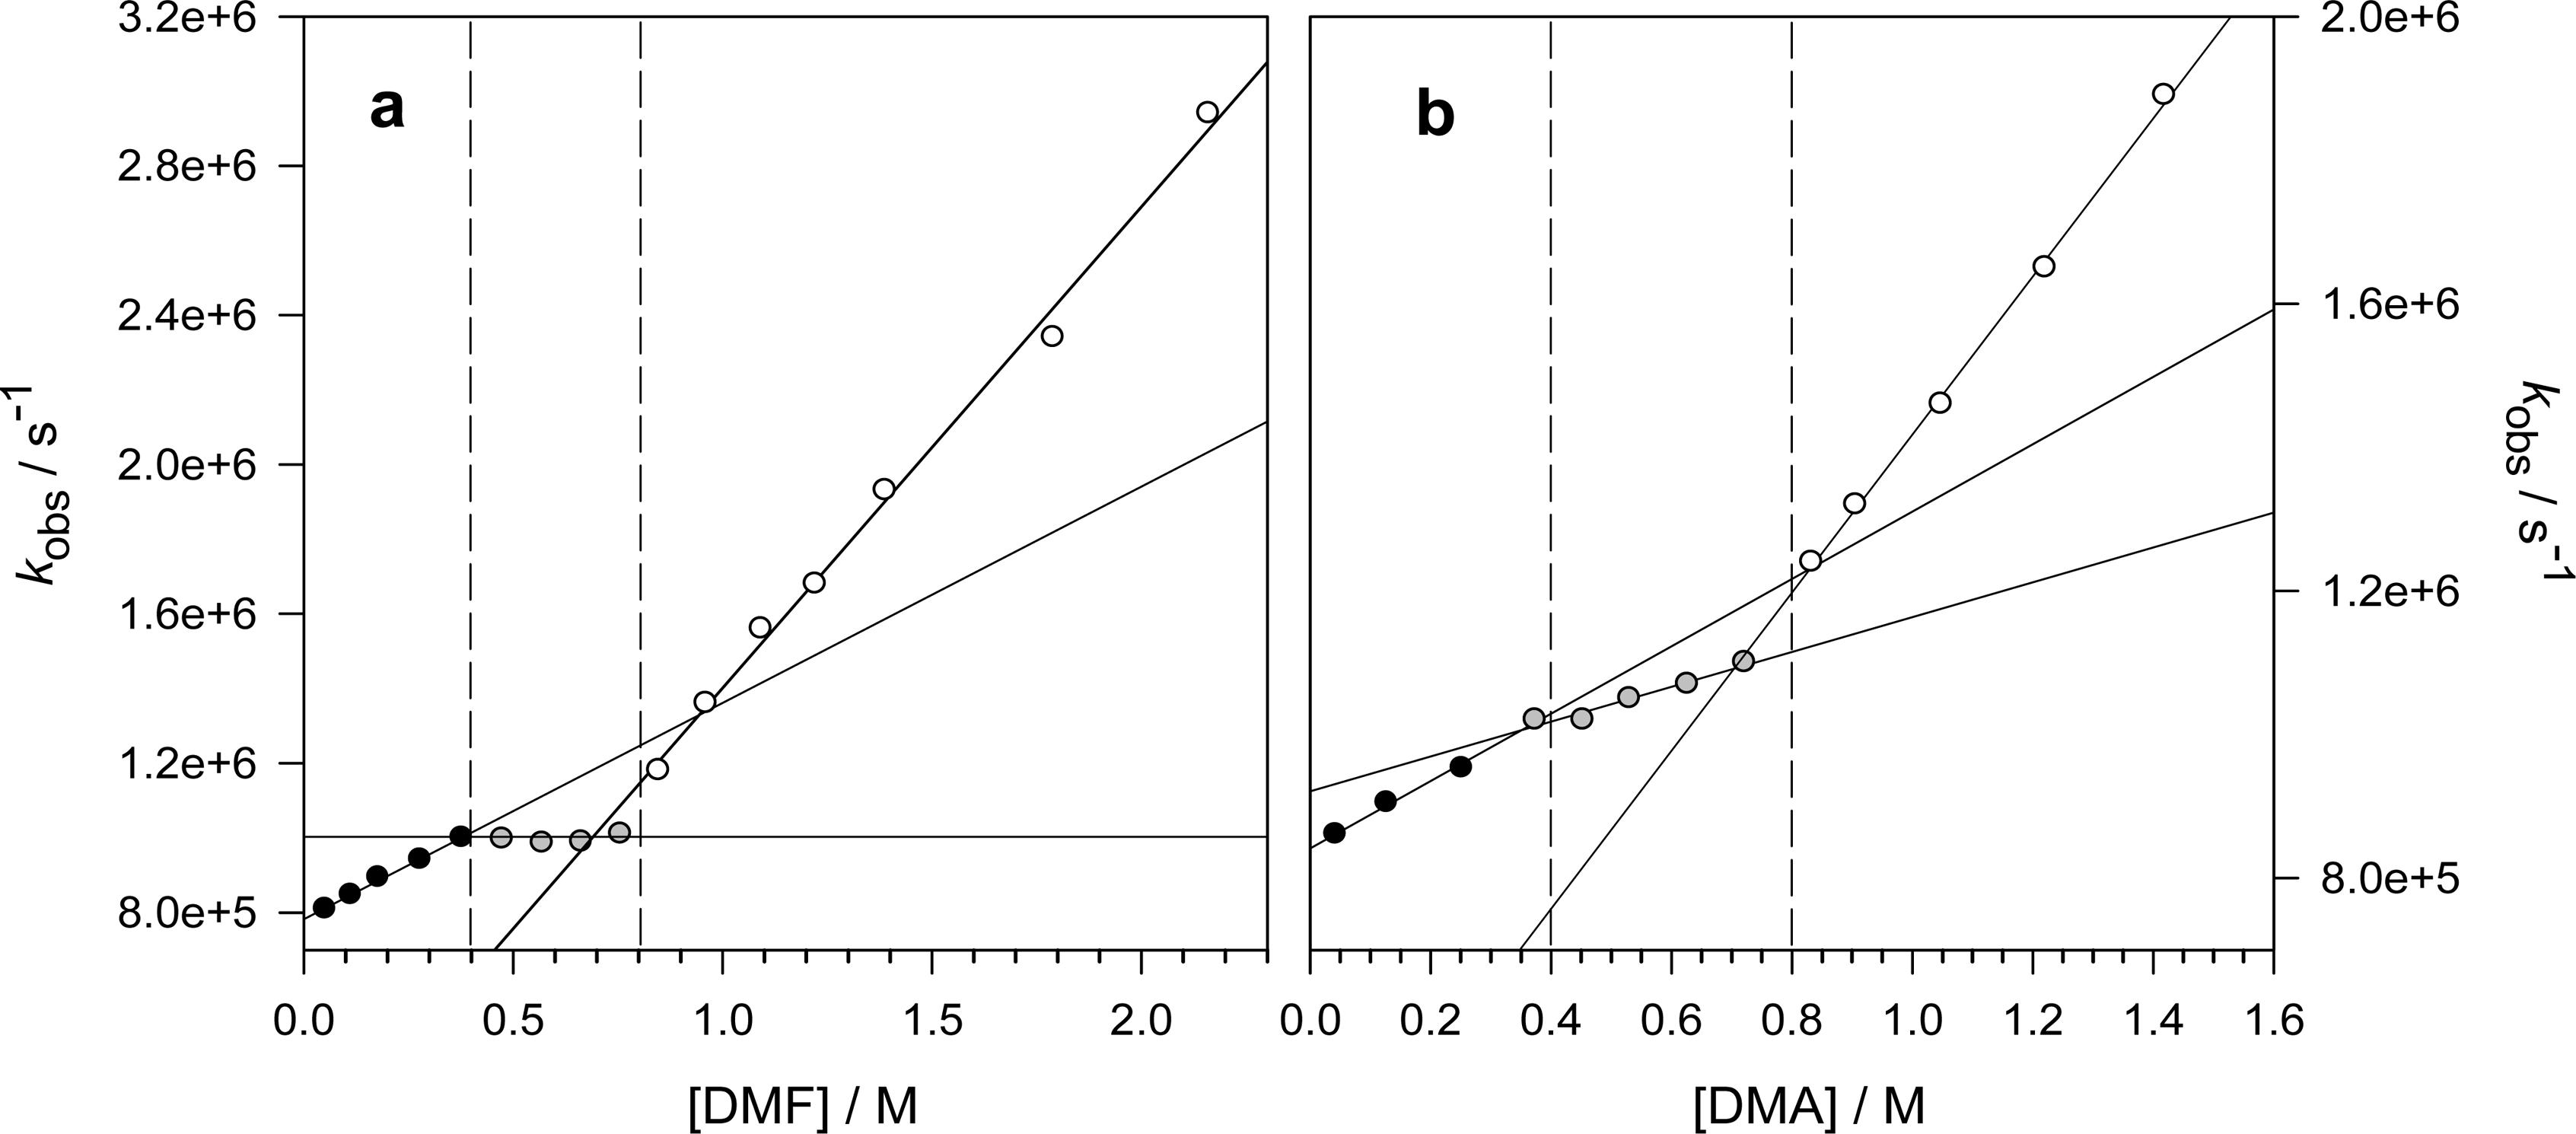
\includegraphics[width=\textwidth]{figures/kH-dma-dmf-mgclo42.png}
  \caption[Plot of observed rate constant against concentration of DMF and DMA
  for reaction with \cumo\ at 298 K in the presence of 0.2 M \ch{Mg(ClO4)2}.]
  {\textbf{a)} Plot of observed rate constant against concentration of DMF for
	  reaction with \cumo\ at 298 K in the presence of 0.2 M
	  \ch{Mg(ClO4)2}. 0--0.4 M [DMF] range (black circles), $k_{H1}$ =
	  5.8\E{5} \Ms; 0.8--2.2 M [DMF] range (white circles), $k_{H2}$ =
	  1.3\E{6} \Ms.  \textbf{b)} Plot of observed rate constant against
  concentration of DMA for reaction with \cumo\ at 298 K in the presence of 0.2
  M \ch{Mg(ClO4)2}. 0--0.4 M [DMA] range (black circles), $k_{H1}$ = 4.7\E{5}
  \Ms; 0.4--0.8 M [DMA] range (grey circles), $k_{H2}$ = 2.4\E{5} \Ms; 0.8--2.2
  M [DMA] range (white circles), $k_{H3}$ = 1.1\E{6} \Ms. Reprinted with
  permission from Reference~\protect\citenum{Salamone2015metals}. Copyright
  2015 American Chemical Society.} \label{fig:k-metals-mg}
\end{figure}

The addition of both \ch{LiClO4} and \ch{LiOTf} decrease to a similar extent
the rate constants for abstraction from DMF and DMA by \cumo. However, in
contrast to \ch{Mg(ClO4)2}, the lithium salts strongly deactivate \ch{C-H}
bonds for 2 equivalents, followed by weak deactivation for another 2
equivalents, and no deactivation for [amide]/[\ch{Li^{+}}]$<$4. Salamone et al.
were not able to give a clear cut explanation, but suggest that the different
patterns are a result of differences in charge density, which is greater for
\ch{Mg^{2+}} than \ch{Li^+}, as well as different coordination geometries of
the two ions. A coordination number of 4 is most common for \ch{Li^+}, while an
octahedral geometry with the coordination of 6 ligands is almost always
observed for \ch{Mg^{2+}}.\cite{Babu2013, Dudev2014} As a result, interactions
of the ions with solvent and counter-anions are suggested to be more important
for \ch{Mg^{2+}} than \ch{Li^+}.

\ch{NaClO4} and \ch{Ca(ClO4)2} influence HAT between \cumo\ and DMA to
different extents than both \ch{LiClO4} and \ch{Mg(ClO4)2}.
\ref{fig:k-metals-naca}a,b shows the plots of $k_{obs}$ against [substrate] for
the reactions of \cumo\ with DMA in MeCN containing 0.2 M \ch{NaClO4} and
\ch{Mg(ClO4)2}, respectively. For \ch{NaClO4}, an almost negligible
deactivation of \ch{C-H} bonds is observed for up to 4 equivalents of DMA. This
was explained on the basis of the weaker Lewis acidity of \ch{Na^+} as compared
to \ch{Li^+}. With regards to \ch{Ca(ClO4)2}, binding to DMA fully deactivates
\ch{C-H} bond abstraction up to 4 equivalents of DMA. The first region
of~\ref{fig:k-metals-naca}b ([DMA] = 0--0.2 M, black circles) represents the
decrease in $k_\beta$ of \cumo\ as \ch{Ca^{2+}} preferentially binds to DMA
over \cumo. Interestingly, for both DMF and DMA, the same experiments in
dimethyl sulfoxide (DMSO) solvent show no inhibition of HAT reactivity by metal
cations. This was rationalized on the basis of the stronger Lewis basicity of
DMSO as compared to both MeCN and the amides, thus the metals preferentially
bind solvent rather than amide substrate.

\begin{figure}[!htbp]
  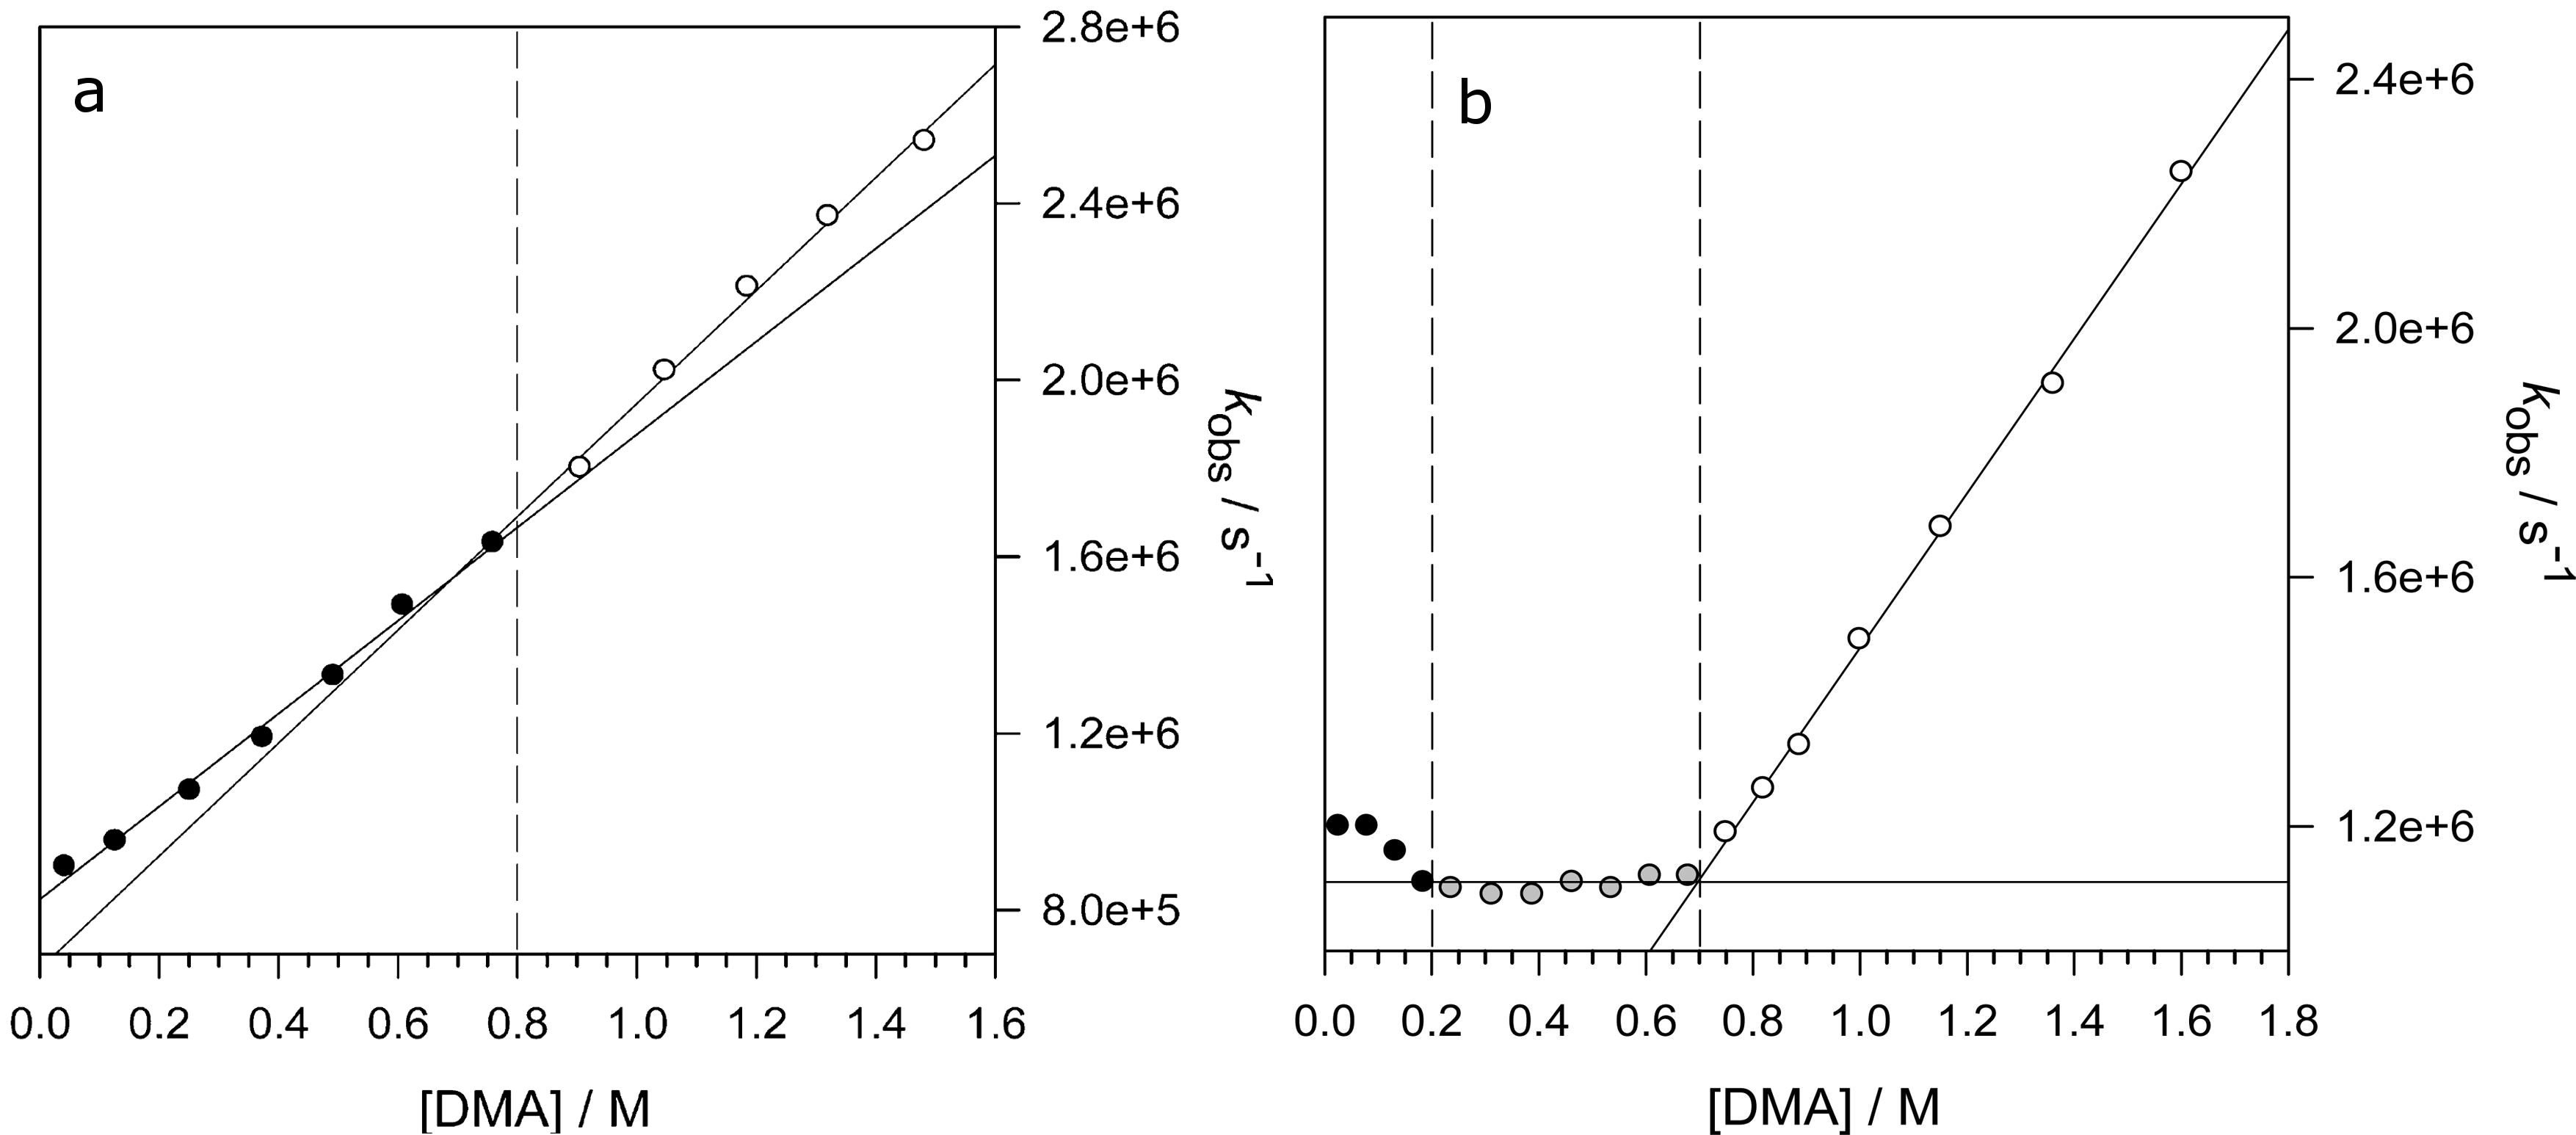
\includegraphics[width=\textwidth]{figures/exptdma-na-ca.png}
  \caption[Plot of observed rate constant against concentration of DMA for
  reaction with \cumo\ at 298 K in the presence of 0.2 M \ch{NaClO4} and
  \ch{Mg(ClO4)2}.] {\textbf{a)} Plot of observed rate constant against
	  concentration of DMA for reaction with \cumo\ at 298 K in the
	  presence of 0.2 M \ch{NaClO4}. 0--0.8 M [DMA] range (black circles),
	  $k_{H1}$ = 9.6\E{5} \Ms; 0.8--1.4 M [DMA] range (white circles),
	  $k_{H2}$ = 1.4\E{6} \Ms.  \textbf{b)} Plot of observed rate constant
  against concentration of DMA for reaction with \cumo\ at 298 K in the
  presence of 0.2 M \ch{Ca(ClO4)2}. 0.8--1.7 M [DMA] range (white circles),
  $k_{H1}$ = 1.2\E{6} \Ms. Adapted with permission from
  Reference~\protect\citenum{Salamone2015metals}. Copyright 2015 American
  Chemical Society.} \label{fig:k-metals-naca}
\end{figure}

Finally, \citet{Salamone2016} examined the effects of substrate structure on
HAT reaction between \cumo\ and sterically bulky tertiary alkanamides in the
presence of alkali and alkaline earth metal ions. For $N,N$-dialkylacetamides,
the steric bulk of the $N$-alkyl groups was previously
characterized.\cite{Salamone2014} Steric repulsion between \cumo\ and the
$N$-alkyl groups can decreases the HAT rate constant, as evident by the 3-fold
decrease in $k_H$ in going from DMA to $N,N$-diisobutylacetamide (DIA; 1.2\E{6}
and 3.1\E{5} \Ms, respectively). For reactions of \cumo\ with DIA addition of
0.2 M \ch{LiClO4} or \ch{Ca(ClO4)2} to results in the same trends in \ch{C-H}
bond deactivation observed for DMA. This indicates that the influence of metal
cation-substrate binding is not significantly influences by the steric bulk of
$N$-alkyl groups.  The same is true for the addition of 0.2 M \ch{Mg(ClO4)2} to
abstraction from DIA by \cumo, as shown in~\ref{fig:k-dia-mg}. Once again, an
slight decrease in reactivity is observed for the first 2 equivalents of DIA,
followed by strong C-H bond deactivation for an additional two equivalents, and
no deactivation beyond that. No additional insight was provided by Salamone et
al. as to the reason for this reactivity. The plausible explanation provided
was once again that \ch{Mg^{2+}} has a high charge density. These results show
that Lewis acid-base interactions between alkali or alkaline earth metal
cations can greatly depress hydrogen abstraction by alkyoxyl radicals.

\begin{figure}[!htbp]
  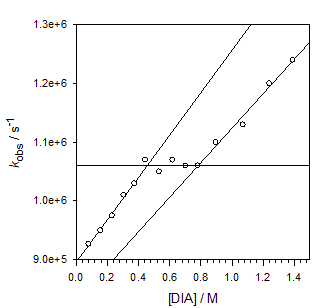
\includegraphics[width=0.6\textwidth]{figures/exptdia-mg.png}
  \caption[Plot of observed rate constant against concentration of DIA for
  reaction with \cumo\ at 298 K in the presence of 0.2 M \ch{Mg(ClO4)2}.]{Plot
	  of observed rate constant against concentration of DIA for reaction
	  with \cumo\ at 298 K in the presence of 0.2 M \ch{Mg(ClO4)2}. 0--0.4
	  M [DIA] range, $k_{H1}$ = 3.6\E{5} \Ms; 0.8--1.4 M [DIA] range,
	  $k_{H2}$ = 2.9\E{5} \Ms.  Reprinted from Tetrahedron, 72, Salamone et
  al., Hydrogen atom transfer from tertiary alkanamides to the cumyloxyl
  radical. The role of substrate structure on alkali and alkaline earth metal
  ion induced \ch{C–H} bond deactivation, 7757--7763, 2016, with permission
  from Elsevier.} \label{fig:k-dia-mg}
\end{figure}

With these results in mind, I am interested in the possibility that alkali and
alkaline earth metal cations found in biological system can protect \ch{C-H}
bonds in proteins from HAT to reactive oxygen-centred radicals. However, the
experimental results do not answer some of the key physico-chemical
determinants which may make this possible. Specifically, I have composed
several important research questions which remain unclear from the experimental
results.

The first question I have is one of methodology: Can DFT-based methods can
accurately treat alkali/alkaline metal cation binding to organic substrates or
radicals? There exists limited ab initio data describing these
interactions.\cite{ Siu2001, Corral2003, Suarez2011, Baldauf2013} Therefore, I
have conducted a benchmark quality study involving \ch{Li^+}, \ch{Na^+},
\ch{Mg^{2+}}, \ch{K^+}, and \ch{Ca^{2+}}. To the best of my knowledge, this
represents the first systematic benchmark study of these metal cations with
both organic substrates and radicals.

Secondly, the nature of the binding of metal ions to substrates is still poorly
described, especially given the odd stoichiometric effects observed for
\ch{Mg(ClO4)2} with alkylamides. Specifically, I wish to address the range of
these interactions, and how much the metals effect the C-H being broken. To
address this I have utilized both \ch{Na^+} and \ch{Mg^{2+}} in my
calculations. These metal ions were chosen to capture the large differences in
Lewis acidity and ion size associated with these third-period ions, and because
they are two of the most biologically relevant metal ions.

Thirdly, I address the effect that metal ions have on the HAT barrier heights.
Experiments demonstrate that under certain conditions, the presence of metal
ions can decrease HAT reactivity. If metal ions do effectively increase C-H
bond strengths, this will be a contributing factor to the free energy barrier
as per the BEP principle\cite{Bell1936,Evans1938} (see Chapter~\ref{ch:bde}).
There will likely be additional factors such as polarization in the TS complex,
or other effects of possible charge transfer from the substrate to metal ions.
To investigate this, I have primarily studied HAT reactions involving DMA and
oxygen-centred radicals. Given there are only experimental data for \cumo, this
is the primary subject, however I was interested in structural differences of
the oxygen-centred radical, thus I have utilized \bno\ as well, which differs
significantly in that it has the ability to form strong pre-reaction complexes
with hydrogen bond accepting substrates.\cite{Salamone2012, Salamone2013} I
also investigated the effect metal cations have on the abstraction from DMA by
the more biologically relevant hydroxyl radical. I have also performed
calculations with the bulkier DIA substrate and \cumo\ to verify whether or not
steric bulk does have an influence on the ability of a metal cation to effect
HAT reactions.

Finally, given that reactions of DMA with \cumo\ in the presence of metal salts
show no deactivation, I was interested in studying the reactivity of alkoxyl
radicals with strong Lewis bases. HAT reactions involving alkoxyl radicals and
strong Lewis bases have been previously studied,\cite{Salamone2012,
vanSanten2016} and can possess interesting and unusual chemical reactivity. For
instance, we recently showed that for the HAT reaction between \bno\ and DMSO,
\bno\ acts as a hydrogen atom donor rather the acceptor.\cite{vanSanten2016} In
light of this, I examined the effect of metal cations on the expected HAT
reactivity between \cumo\ and DMSO, as well as the ``reverse'' HAT reactivity
between \bno\ and DMSO. I also performed calculations to determine the effects
of metal cations and if there exists reverse reactivity for two other strong
Lewis basic substrates: hexamethylphosphoramide (HMPA) and tributylphosphine
oxide (TBPO). The chemical structures of all the species studies herein are
shown in~\ref{fig:hat-subs}.

\begin{scheme}[!htbp]
  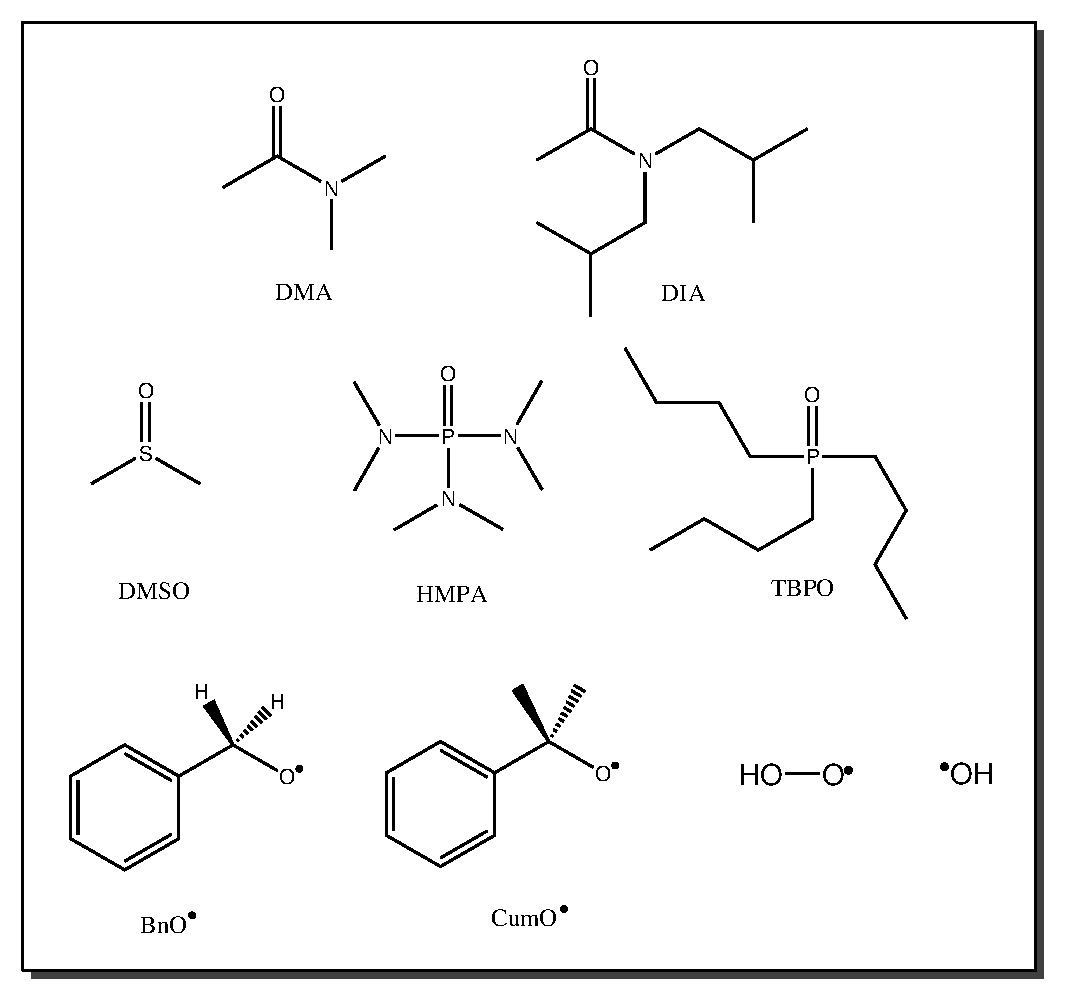
\includegraphics[width=\textwidth]{figures/Substrates.eps}
  \caption{Chemical structures of the species studies herein.}
  \label{fig:hat-subs}
\end{scheme}


\section{Computational methods and details}

All quantum mechanical calculations were performed using either the Gaussian 09
software package,\cite{Frisch2009} or the TURBOMOLE software
package.\cite{turbomole} Calculations for the benchmark quality data of metal
binding to substrates were first optimized at the
LC-$\omega$PBE-D3(BJ)/6-31+G(2d,2p) level of theory,\cite{Vydrov2006,
Vydrov2006a, Grimme2010, Johnson2006} and later re-optimized with larger
6-311+G(3df,3pd) basis sets. Single-point energy calculations were then carried
out using the coupled cluster methodology with single, double and perturbative
triples with full core correlation, CCSD(T,Full), and various basis sets, as
will be described in Section~\ref{sec:benchmark}. Final benchmark quality
binding energies have been calculated using the F12$^*$ explicitly correlated
method with Def2-QZVPPD primary basis sets and Def2-QZVPP auxiliary basis sets
required for the resolution-of-the-identity (RI) approximation as implemented
in TURBOMOLE. The RI approximation is used to reduce the computational cost
associated with calculating MO integrals.\bibnote{For a detail description of
the RI approximation and explicit correlation, see
Ref.~\protect\citenum{OterodelaRoza2017}, Chapter 4.} A total of 31 different
DFT-based methods with nearly complete 6-311+G(3df,3pd) and moderate sized
6-31+G(2d,2p) basis sets were tested both by single-point energy calculations
on the benchmark structures. Geometry optimization calculations starting from
the benchmark structures were also performed for three of the best performing
DFT-based method, in order to verify their ability to capture the minimum
energy bound structures.

To test the effects of metal cations on HAT barrier heights, calculations were
first performed for the reactions not involving metal cations. Geometry
optimizations were performed at the M05-2X\cite{Zhao2006}/6-31+G$^{**}$ level
of theory. Transition state (TS) structures were obtained by first freezing the
abstraction donor-hydrogen-acceptor bond lengths with multiple initial
orientations. The frozen bonds were then relaxed to obtain the final TS
structures, which were then used to identify the appropriate pre- and
post-reaction complexes. All structures were subjected to harmonic vibrational
frequency calculations, which were visualized using the Chemcraft
program\cite{ccraft} to verify minima (or saddle-points with a single imaginary
frequency connecting reactants to products for TS structures). Single-point
energy calculations were performed at the M05-2X/6-311+G(2d,2p) level of
theory. The effects of MeCN solvent were estimated by inclusion of the
SMD\cite{Marenich2009} continuum solvent model in single-point energy
calculations.

The inclusion of metal cations into the TS structures proved to be technically
challenging. It was my expectation that I could simply include metal cations
and necessary counter-anions into the minimum energy complex structures and
re-optimize, however this was not the case. TS structures were once again
obtained by constrained optimization with the inclusion of the metal cation and
counter-anion and freezing the abstraction donor-hydrogen-acceptor bond
lengths, providing a guess TS structure. However, in most cases the force
constants (which are necessary for a TS optimization calculation) from the
guess TS structure were not representative of the true TS structure, thus force
constants were recalculated for every step along the optimization, using the
``CalcAll'' keyword in Gaussian. This is a very computationally expensive
procedure. Even using this method, many TS structures including metal cations
failed to converge. Therefore, guess TS structures which contain a single
imaginary frequency connecting reactants to products are used in place. This
technique provides genuine TS structures, although they may not be the TS
associated with the minimum energy reaction pathway. Nonetheless, the guess TS
structure can be used provide an estimate of the reaction barrier height which
are verified with calculations that were successful. Where available, final TS
structures were used to identify the appropriate pre- and post-reaction
complexes.

Natural bond order (NBO) and natural population analysis (NPA) were utilized in
order to investigate the electronic structures involved in the HAT reactions
and the effects of metal cation binding.\cite{Reed1983, Reed1985,
Glendening2012} Version 3.1 of the NBO software package,\cite{NBO3} as
implemented in the Gaussian 09 package was used in all cases.\cite{Frisch2009}
NBO analysis provides a means for estimating the physical effects of chemically
intuitive orbital interactions while NPA charges are a means for calculating
the occupancies and charges of atomic centres.\cite{Landis2014, Weinhold2016}

\sectionmark{Benchmarking DFT based methods}
\section{Benchmarking DFT based methods for the binding of alkali and alkaline
earth metals to organic substrates and oxygen centred radicals}
\sectionmark{Benchmarking DFT based methods}
\label{sec:benchmark}

In order to confidently perform quantum mechanical mechanistic studies, the
method of choice must be calibrated. While DFT-based methods have been widely
applied to these studied, few studies have previously investigated alkali and
alkaline earth-metal cation binding to organic substrates.\cite{Corral2003,
Suarez2011, Siu2001, Baldauf2013} Most importantly, benchmark quality data for
a wide variety of metals binding to biologically relevant substrates and
oxygen-centred radicals does not exist to calibrate DFT-based methods.
Therefore, I proposed a benchmark study which incorporated all the biologically
relevant alkali and alkaline earth-metal cations, models for dipeptides
including amino acid side chains, oxygen-centred radicals, and solvents which
are utilized in the experimental mechanistic studies involved in probing these
systems. Unfortunately, due to computational restrictions (\emph{vide infra}),
benchmark quality calculations on the originally proposed benchmark set were
not possible. Full details of the originally proposed benchmark set are in
Appendix~\ref{ap:hat},~\ref{fig:ap-set1}.

Benchmark quality binding energies are generally calculated using the ``gold
standard'' approach, CCSD(T)/CBS, where correlation consistent basis
sets\cite{Marshall2011, Rezac2013} (cc-pV\emph{X}Z, \emph{X}=T,Q,5) developed
by Dunning and\cite{Vydrov2006, Vydrov2006a} co-workers are used for complete
basis set extrapolation. For the alkali and alkaline earth-metals,
\citet{Iron2003} demonstrated that additional $d$-type basis functions are
necessary to obtain reasonable results. It is also necessary to include
core-correlation of at least the first core shell in alkali and alkaline earth
metals, thus it would be appropriate to use core valence basis sets such as
cc-pCV$X$Z.\cite{Peterson2002} \citet{Iron2003} also developed core-valence
basis sets for the alkali and alkaline earth-metals, however I was not able to
obtain these basis sets until very recently.\bibnote{See
http://theochem.weizmann.ac.il/web/papers/group12.html for the CV$N$Z  basis
sets for Li, Be, Na, Mg, K, Ca.} These basis sets should be considered for
future benchmarking work. Given these difficulties, I originally chose the
augmented version of the polarization consistent basis sets of Jensen and
co-workers\cite{Jensen2001, Jensen2002, Jensen2002a, Jensen2003}
(aug-pc-\emph{N}, \emph{N}=2,3,4), which have been shown to converge to the CBS
limit systematically\cite{Kupka2007} and are available for all the elements of
interest.

While performing CCSD(T)/CBS calculations, I observed that the metal cations
(and neutral metal atoms), did not converge smoothly to the complete basis set
limit. As a consequence, complete basis set extrapolation is not feasible. In
light of this problem, I decided to re-evaluate the size scope of the benchmark
set being used. In order to facilitate future DFT-based work and probe the
issue of basis set convergence of alkali and alkaline earth metals, a benchmark
set of small substrates was proposed. This new set is shown in \ref{fig:set2}.
The new, small benchmark set was selected to include important functional
groups and radicals found biological systems, and one of the most common
solvents used in physical organic experiments, acetonitrile.

\begin{scheme}[!htbp]
  \centering
    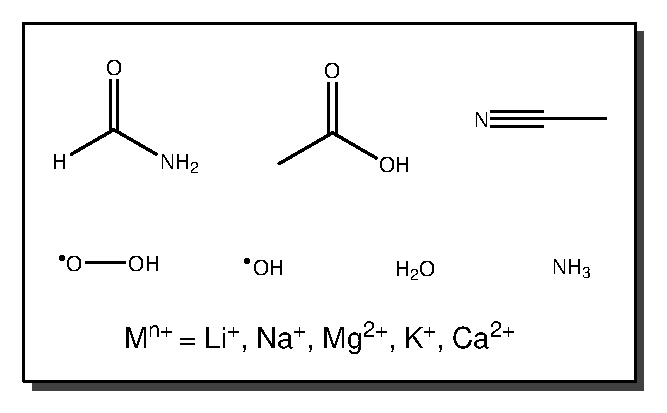
\includegraphics[width=\textwidth]{figures/set2.eps}
    \caption{Revised benchmark set of small substrates and cations. Note this
    set consists of all combinations of substrates and metal cations, i.e.,
    there are 35 complexes in the set.} \label{fig:set2}
\end{scheme}

\subsection{Metal cation basis set convergence}

\begin{figure}[!htbp]
  \centering
    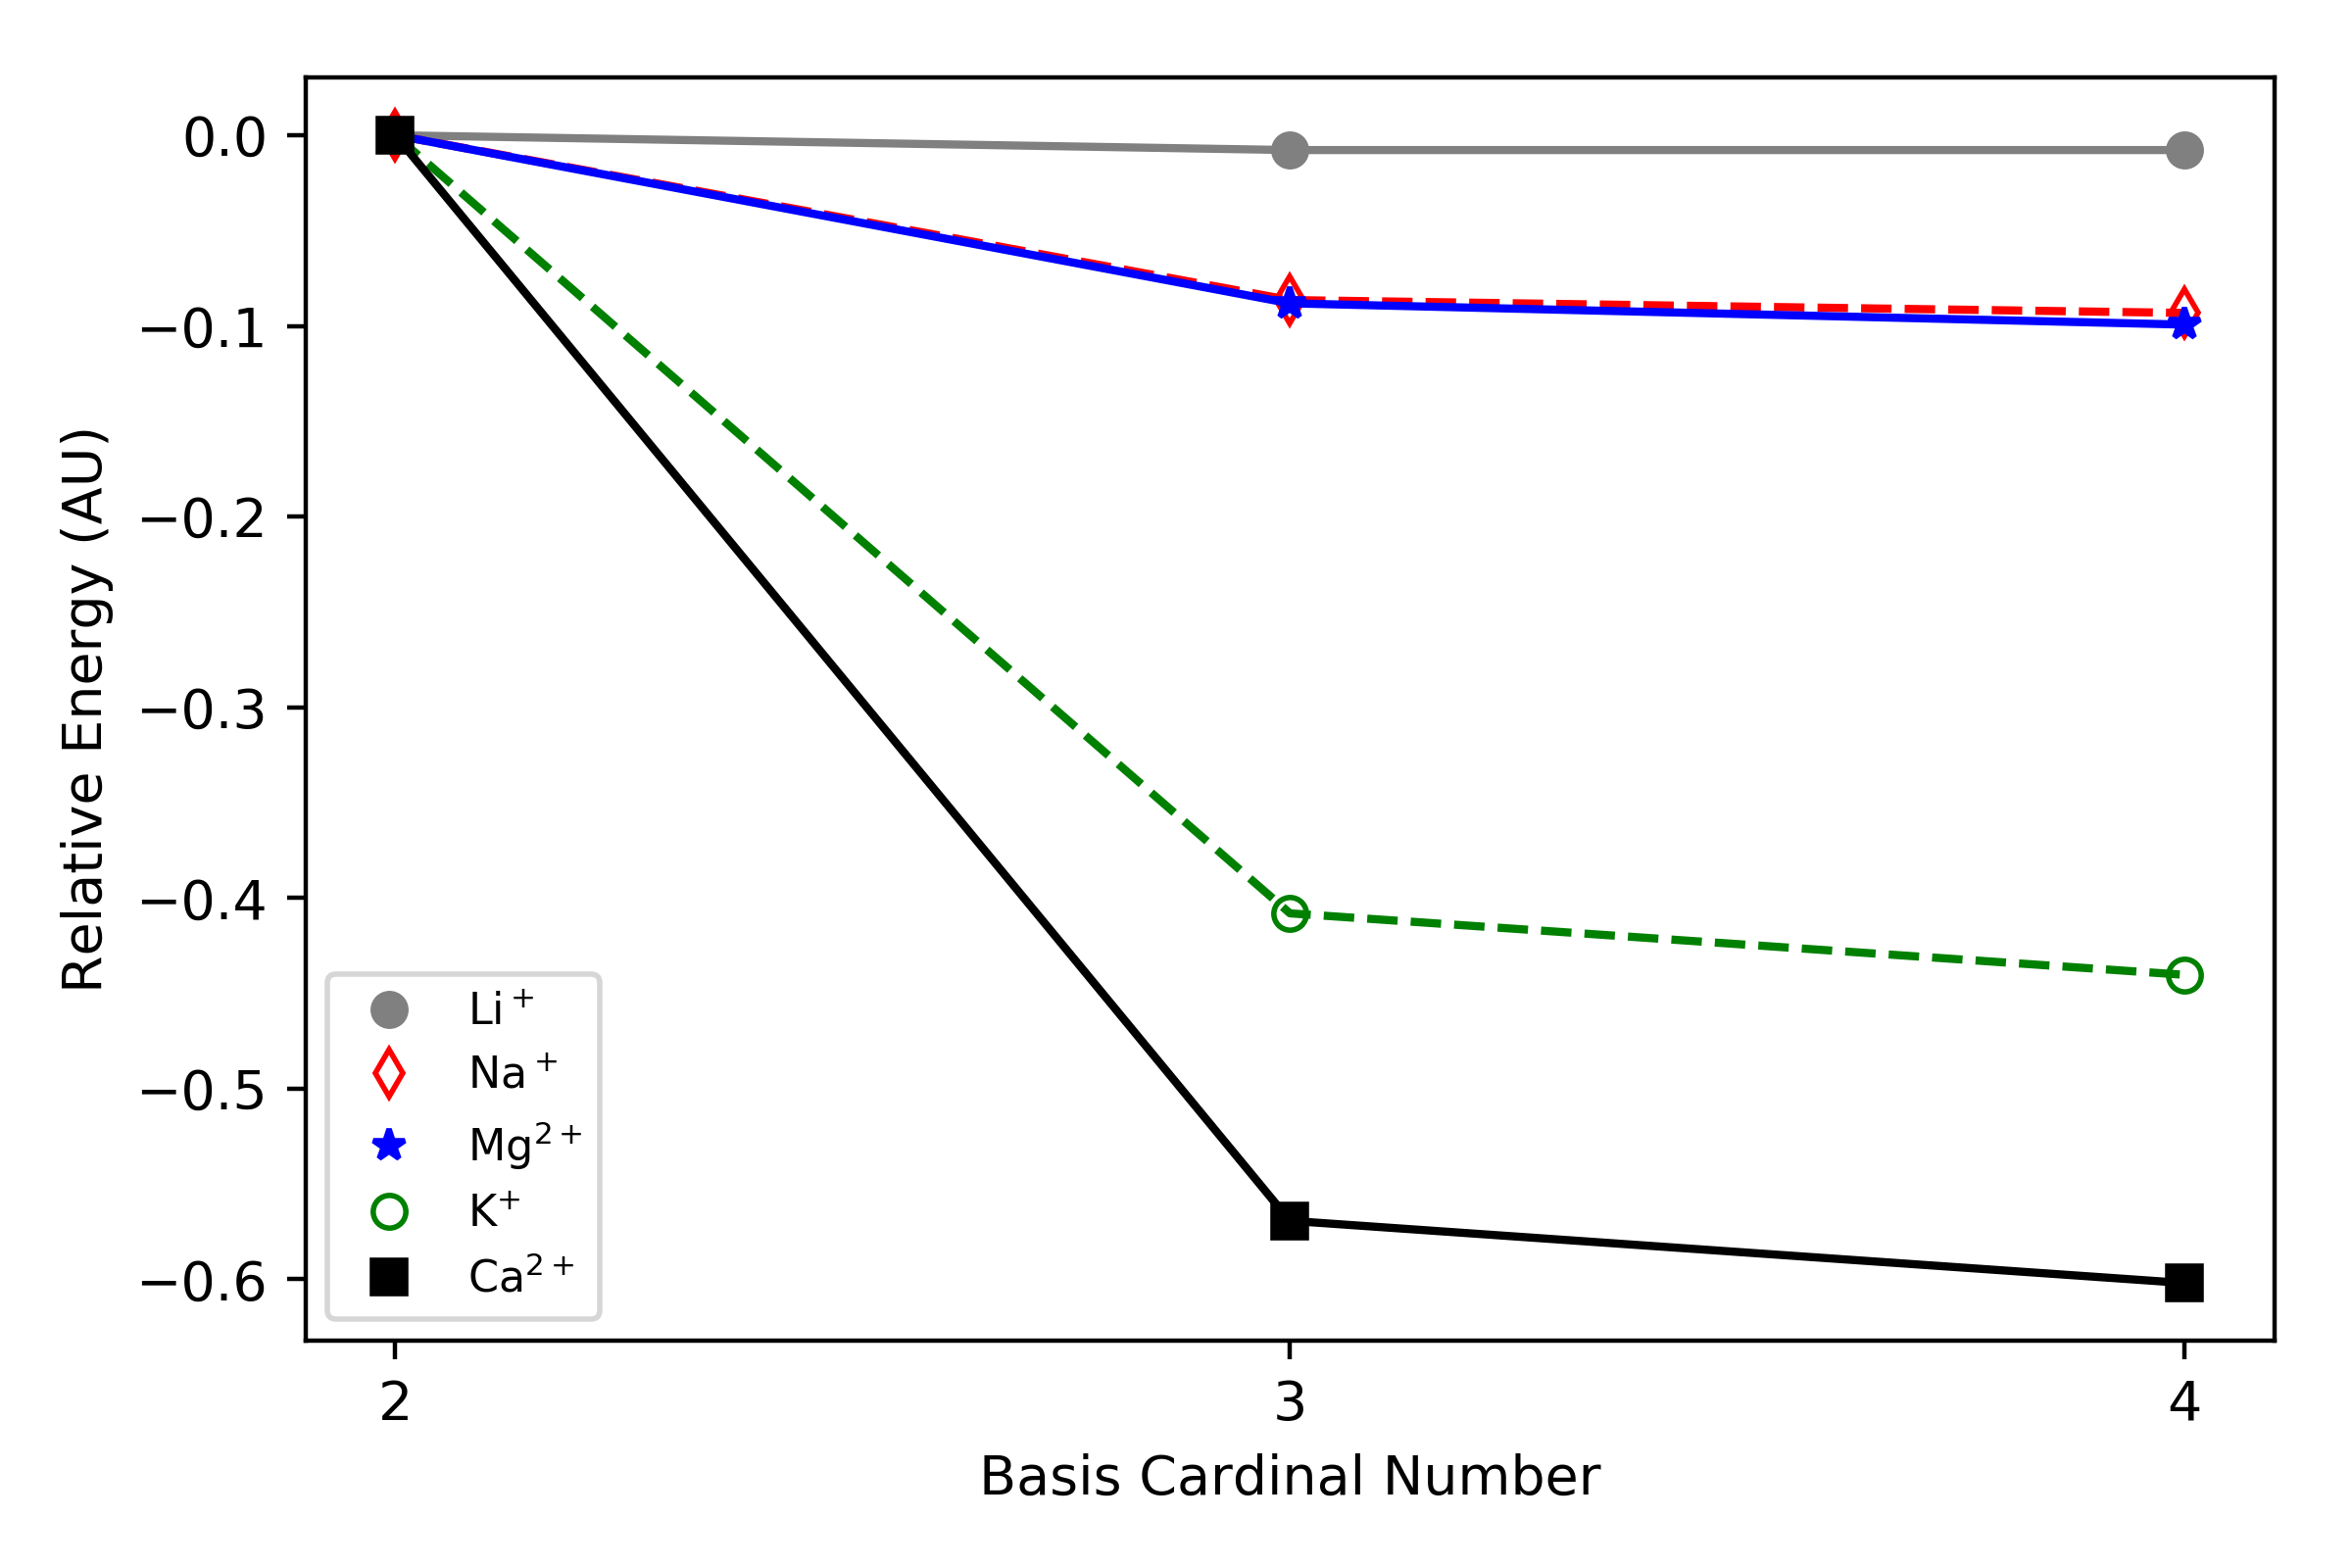
\includegraphics[width=\textwidth]{figures/ap_metals_explicit}
    \caption[Explicitly correlated basis set convergence for alkali and
    alkaline earth-metal cations.]{Explicitly correlated
    CCSD(T,Full)-F12$^*$/Def2-$X$ ($X$=SVP,TZVPPD,QZVPPD) basis set convergence
    for alkali and alkaline earth-metal cations. The relative energy of each
    basis set relative to the Def2-SVP for each metal. The cardinal number of
    the basis sets is $X$.} \label{fig:metals_explicit}
\end{figure}

In order to perform complete basis set (CBS) extrapolation, the total energy of
a molecule/atom should converge smoothly to the CBS limit.\cite{Truhlar1998}
However, CCSD(T,Full)/aug-pc$N$ ($N$=1,2,3,4) calculations for alkali and
alkaline earth-metals convergence of poorly to the CBS limit (See
Appendix~\ref{ap:hat}, ~\ref{fig:pes_metals}). Examining the energy of each ion
relative to the smallest basis set, for \ch{Li^+} the value appears to converge
reasonably, however this because there are only 2 electrons in this ion. For
all of \ch{Na^+}, \ch{Mg^{2+}}, \ch{K^+}, and \ch{Ca^{2+}}, there appears to be
no convergence to the CBS limit as each line continues down linearly. This is
problematic as it means that CBS extrapolation would result in a significant
degree of uncertainty in the estimated CBS limit total energy.

The poor convergence was thought to be a result of poorly suited basis sets to
full core-correlation. However, the same CCSD(T,Full) calculations using the
core-correlation (cc-pCV$N$Z) basis sets also show unsatisfactory convergence
for \ch{Na^+} and \ch{Mg^{2+}} (See Appendix~\ref{ap:hat},
~\ref{fig:ap_pes_metals}). Therefore, I was tasked with finding a method which
would give results which best approximate alkali and alkaline metal binding at
the complete basis set limit. I decided to use an explicitly correlated CCSD(T)
treatment known as ``F12$^*$'' to more rapidly approach the CBS
limit.\cite{Tenno2012} I tested both the core-correlation consistent basis set
developed for used with explicitly correlation
(cc-pCV$X$Z-F12),\cite{Peterson2008} and the Ahlrich basis sets
(Def2-SVP,-TZVPPD, and -QZVPPD).\cite{Rappoport2010} Both these basis sets
combined with the CCSD(T,Full)-F12$^*$ methodology gave satisfactory
convergence to the CBS limit for the sodium and magnesium ion
(see~\ref{fig:metals_explicit}) for the convergence of all metal ions
calculated with the CCSD(T,Full-F12$^*$/Def2-QZVPPD method). Given that
Def2-QZVPPD is available for almost every atom on the periodic table, and the
observed convergence to the CBS limit, this basis set was selected for
benchmark quality binding energies.

To the best of my knowledge, there is no precedent for extrapolating the
Ahlrich basis sets, thus the final benchmark energies are at the
CCSD(T)-F12$^*$/Def2-QZVPPD level of theory, without extrapolation. The
convergence of the total energies of the cations can be estimated as the sum of
the experimental ionization energies of the ions. These results are listed
in~\ref{tab:metal-energy}. The calculated values are too high (i.e., not at the
CBS limit), and deviate from experiment from 0.16 and 0.66 AU (4.4--18 eV).
Deviations of this magnitude are rather significant, and are likely due to the
increasing contribution of ``relativistic effects'' with increasing atomic
number. Additionally, there may be cumulative experimental error, as the
experimental ionization energies range from 4--5500 eV. Relativistic effects
were not considered herein, thus, the calculated binding energies herein are
likely the best available approximation to the non-relativistic gas-phase
metal-substrate binding energy.

\begin{table}[!htbp]
  \caption[Total energy of alkali and alkaline earth-metal cations.]{Total
  energy of alkali and alkaline earth-metal cations from experimental
  ionization energies\cite{CRC2016} (Expt.) and calculated (Calc.) at the
  CCSD(T,Full)-F12$^*$/Def2-QZVPPD level of theory. All values are in units of
  AU.} \label{tab:metal-energy}
  \begin{tabular}{l c c}
    \textbf{Ion} & \textbf{Expt.} & \textbf{Calc.} \\
    \hline
    \ch{Li^+} & -7.47798 & -7.27983 \\
    \ch{Na^+} & -162.43089 & -162.24203 \\
    \ch{Mg^{2+}} & -200.32523 & -199.49171 \\
    \ch{K^+} & -601.93332 & -601.77381 \\
    \ch{Ca^{2+}} & -680.19158 & -679.53065
  \end{tabular}
\end{table}

\subsection{High level results and evaluation of various density-functional theory based methods}

\ref{tab:ccsd-metal} lists the benchmark binding energy values calculated at
the CCSD(T,Full)-F12$^*$/Def2-QZVPPD//LC-$\omega$PBE-D3(BJ)/6-311+G(3df,3pd)
level of theory. Some general trends are that alkaline earth-metals bind more
strongly than alkali earth-metals. Also, the order of binding follows the Lewis
acidity of the metal ions: \ch{Mg^{2+}} $>$ \ch{Ca^{2+}} $>$ \ch{Li^+} $>$
\ch{Na^+} $>$ \ch{K^+}. The metals all appear to bind most strongly to the
amidic oxygen-centre, reflecting the higher Lewis basicity. The metals also
bind weakest to the oxygen-centred radicals, with greater binding to \ch{HOO^.}
as compared to \ch{HO^.}.

\begin{table}[!htbp]
  \caption[Benchmark gas-phase binding energies of alkali and alkaline
  earth-metals with small organic substrates and radicals.]{Benchmark gas-phase
  binding energies of alkali and alkaline earth-metals with small organic
  substrates and radicals. Values are calculated at the
  CCSD(T,Full)-F12$^*$/Def2-QZVPPD//LC-$\omega$PBE-D3(BJ)/6-311+G(3df,3pd)
  level of theory. All values are in \kcalmol.}\label{tab:ccsd-metal}
  \begin{tabular}{l c c c c c}
            &\ch{Li^+}&\ch{Na^+}&\ch{Mg^{2+}}&\ch{K^+}&\ch{Ca^{2+}}\\
    \hline
    \ch{H2O}    & -34.7 &  -24.4 &  -82.0  &  -17.8 &  -56.8 \\
    \ch{NH3}    & -39.9 &  -28.2 &  -98.1  &  -19.8 &  -65.3 \\
    MeCN        & -44.4 &  -33.0 &  -113.1 &  -24.9 &  -80.7 \\
    Formamide   & -50.7 &  -36.9 &  -128.2 &  -28.5 &  -96.1 \\
    Formic acid & -38.4 &  -27.0 &  -101.9 &  -20.0 &  -72.6 \\
    \ch{HO^.}   & -21.3 &  -16.8 &  -57.0  &  -12.4 &  -40.7 \\
    \ch{HOO^.}  & -27.1 &  -19.1 &  -72.2  &  -13.9 &  -49.0
  \end{tabular}
\end{table}

Next, 31 DFT-based methods combined with a moderate basis set (6-31+G(2d,2p))
and a large basis set (6-311+G(3df,3pd)) were tested for their ability to
estimate the binding energy between metal cations and substrates. The mean
absolute/signed errors (MAE/MSE) and maximum and minimum errors for each method
are listed in~\ref{tab:dft-metal}.

\setlength\LTleft{-1cm}
\begin{longtable}[!htbp]{m{4cm} c c | c c}
\caption[Evaluation of DFT-based methods for alkali and alkaline metal binding
to organic substrates and radicals.]{Evaluation of DFT-based methods for alkali
and alkaline metal binding to organic substrates and radicals. All values are
in \kcalmol. Negative values indicate under-binding.} \label{tab:dft-metal}\\
\textbf{Method}&\textbf{MAE/MSE}&\textbf{Max./Min}&\textbf{MAE/MSE}&\textbf{Max./Min.}\\
\hline
 & \multicolumn{2}{c|}{6-311+G(3df,3pd)} & \multicolumn{2}{c}{6-31+G(2d,2p)}\\
B3\cite{Becke1993}LYP\cite{Lee1988} &  1.49/1.35 &  5.12/-0.57  &  1.59/-0.17 &  4.67/-7.28 \\
B3P86\cite{Perdew1986} &  0.94/0.47 &  3.87/-0.96  &  1.36/-1.08 &  1.99/-7.38 \\
B3PW91\cite{Perdew1991}  &  0.95/-0.14 &  2.74/-1.64  &  1.89/-1.70 &  1.47/-8.76 \\
BH+H\cite{Becke1993a}LYP &  1.89/1.84 &  5.29/-0.59  &  1.93/0.63 &  4.65/-5.64 \\
B\cite{Becke1988}LYP  &  1.60/1.07 &  5.56/-1.51  &  1.88/-0.75 &  5.30/-8.80 \\
BMK\cite{Boese2004}   &  0.90/-0.70 &  1.13/-2.40  &  1.98/-1.93 &  0.86/-8.75 \\
BP86              &  1.63/-0.25 &  4.61/-3.21  &  2.27/-2.14 &  1.55/-9.38 \\
CAM-B3LYP\cite{Yanai2004} &  2.40/2.40 &  6.25/ 0.21  &  1.98/1.04 &  5.82/-5.25 \\
LC-$\omega$PBE\cite{Vydrov2006, Vydrov2006a} &  0.78/0.58 &  2.95/-0.73  &  1.34/-0.74 &  2.19/-8.00 \\
M05-2X\cite{Zhao2006} &  1.11/1.11 &  3.21/ 0.15  &  1.24/-0.17 &  2.55/-5.75 \\
M06\cite{Zhao2008}    &  1.05/-0.62 &  2.36/-4.83  &  1.83/-1.63 &  1.76/-9.03 \\
M06-2X\cite{Zhao2008} &  1.13/1.13 &  3.68/ 0.11  &  1.26/-0.07 &  3.00/-6.63 \\
M06L\cite{Zhao2006b} &  1.52/-1.14 &  2.64/-6.94  &  2.55/-2.48 &  1.21/-11.2 \\
MOHLYP\cite{Schultz2005} &  2.30/-2.02 &  1.52/-5.40  &  4.04/-3.96 &  0.89/-15.2 \\
PBE0\cite{Adamo1999, Ernzerhof1999} &  1.22/1.18 &  4.19/-0.31  &  1.25/-0.34 &  3.30/-7.25 \\
PBE\cite{Perdew1996} &  1.70/1.46 &  6.09/-0.87  &  1.58/-0.46 &  4.68/-8.15 \\
TPSS\cite{Tao2003}   &  1.38/0.95 &  4.88/-1.12  &  1.60/-0.98 &  2.91/-8.12 \\
B97\cite{Becke1997}D3\cite{Grimme2010} &  1.50/0.47 &  5.94/-2.19  &  1.69/-1.37 &  2.67/-8.41 \\
$\omega$B97\cite{Chai2008a} &  0.61/0.23 &  2.13/-1.72  &  1.41/-0.97 &  1.78/-7.57 \\
$\omega$B97XD\cite{Chai2008} &  1.12/-0.94 &  1.02/-4.52  &  2.24/-2.21 &  0.65/-8.64 \\
HSEH1PBE\cite{Heyd2004, Heyd2005} &  1.30/1.29 &  4.28/-0.16  &  1.23/-0.23 &  3.45/-6.95 \\
B3LYP-D3(BJ)\cite{Grimme2010, Johnson2006} &  2.86/2.86 &  7.50/ 0.34  &  1.92/1.34 &  7.05/-4.33 \\
BLYP-D3(BJ)       &  2.89/2.88 &  8.40/-0.14  &  1.83/1.06 &  8.14/-5.30 \\
B3PW91-D3(BJ)     &  1.47/1.40 &  5.81/-0.44  &  1.02/-0.14 &  3.88/-5.69 \\
BMK-D3(BJ)        &  1.03/0.80 &  4.05/-1.06  &  1.02/-0.43 &  2.03/-5.49 \\
BP86-D3(BJ)       &  1.77/1.29 &  7.78/-1.05  &  1.26/-0.60 &  3.96/-6.19 \\
CAM-B3LYP-D3(BJ)  &  3.19/3.19 &  7.50/ 0.78  &  2.27/1.82 &  7.07/-3.54 \\
LC-$\omega$PDE-D3(BJ)& 1.47/1.46 & 4.07/-0.06 &  1.33/0.14 &  3.30/-6.15 \\
PBE0-D3(BJ)       &  1.92/1.92 &  5.37/ 0.20  &  1.33/0.40 &  4.47/-5.74 \\
PBE-D3(BJ)        &  2.24/2.23 &  7.57/-0.22  &  1.44/0.30 &  5.90/-6.67 \\
TPSS-D3(BJ)       &  2.03/1.99 &  6.93/-0.30  &  1.25/0.06 &  4.56/-6.03
\end{longtable}
\setlength\LTleft{0pt}
\setlength\LTright{0pt}

Given the magnitude of the binding energies, the overall agreement between the
benchmark values and the DFT-based method values with both moderate and large
basis sets is very good. Interestingly, the application of the empirical D3(BJ)
dispersion correction systematically decreases agreement with benchmark values
as it increases over-binding. Also, going from moderate to large basis sets
systematically increases the predicted binding energies, as indicated by an
increase in MSE across the board. I chose three of the best performing methods
(BMK-D3(BJ), TPSS-D3(BJ), and M05-2X) and performed geometry optimizations with
moderate basis sets on the reference structures to determine if the choice of
method would significantly impact the minimum energy bound structure. These
results are listed in~\ref{tab:ccsd-metal-opt}.

\begin{table}
  \caption[Comparison of single point and relaxed binding energies for alkali
  and alkaline metal binding with DFT-based methods.]{Comparison of single
  point (SP on benchmark structure) and relaxed (optimized with method) binding
  energies for alkali and alkaline metal binding with DFT-based methods and
  6-31+G(2d,2p) basis sets. Mean absolute error (MAE) values are in \kcalmol\
  and average root mean squared deviation (RMSD)\bibnote{Root mean square
  deviation was calculated using the Kabsch algorithm\protect\cite{Kabsch1976}
  as implemented in the rmsd package available on GitHub (Calculate RMSD for
  two XYZ structures, GitHub, http://github.com/charnley/rmsd, accessed Nov.
  18, 2016)} of geometry are in \AA.}\label{tab:ccsd-metal-opt}
  \begin{tabular}{l c c c}
    Method & MAE(SP) & MAE(Relaxed) & Average RMSD \\
    \hline
    BMK-D3(BJ) & 1.02 & 1.24 & 0.012 \\
    M05-2X & 1.24 & 1.17 & 0.020 \\
    TPSS-D3(BJ) & 1.25 & 1.21 & 0.026 \\
  \end{tabular}
\end{table}

For all the three methods tested, the average of the root mean square
deviations (RMSD) from reference structures are very small (0.012--0.026 \AA).
For BMK-D3(BJ), re-optimization of the structures results in a slight increase
in MAE, while for TPSS-D3(BJ) and M05-2X, the opposite is true. As a whole, it
seems that DFT-based methods are capable of predicting gas-phase binding
energies for alkali and alkaline metal ions with organic substrates and
radicals. M05-2X appears to be one of the best performing DFT-based methods.
Furthermore, M05-2X is recommended by the QM-ORSA\cite{Galano2013} method,
which outlines ``best principles'' for calculating accurate HAT rate constants
in solution. And finally, M05-2X was previously used by our group in the study
of the HAT reaction between DMSO and \bno,\cite{vanSanten2016} thus I have
selected this method for further study of the effects of alkali and alkaline
earth metal cations on the barrier heights of HAT reactions. Note also that
M05-2X is a hybrid density-functional with 56\% HF-exchange, and thus should
not suffer significantly from delocalization error.

\section{Exploring the nature of metal cation substrate interactions}

The first step to understanding the effect non-redox active metal have on HAT
reaction barrier heights is investigating the nature of the binding
interaction. \ref{fig:pes-dma-na}a,b show the potential energy surfaces (PESs)
of the binding of sodium ion, and sodium chloride to DMA, respectively. There
are three surfaces in each plot representing the same potential energy surface
in the gas-phase (black circles), and in an SMD\cite{Marenich2009} continuum
solvent field of MeCN (grey squares) or water (white circles). For both sodium
ion and sodium chloride, the gas-phase PES demonstrates severe over-binding
with respect to a solvated system. This is indicated by a much deeper well than
both solvents and a long-range interaction that does not tail off within 6
\AA\ due to the lack of screening. This simply underscores the importance
of including solvent effects in studying the effects of metal cations.
Interestingly, for the effects of water compared to MeCN solvent appears to be
quite small. In both cases the difference between the minimum of the water PES
is about 2.5 \kcalmol, while the differences in range of interaction is
negligible. Furthermore, the minimum of the PES well in all cases falls at
about the same distance (2.1--2.2 \AA) in the gas-phase and in both solvents.
The small differences in binding interactions indicate that the effects as
measured in MeCN should also apply to the more biologically relevant aqueous
system. 

For both the ion and the salt of sodium in water and MeCN, the binding
interaction only approaches zero. Even at 6 \AA, the predicted binding energy
of DMA in water with \ch{Na^+} and \ch{NaCl} are 1.1 and 0.7 \kcalmol,
respectively. This is an indication that M05-2X-SMD does not properly capture
long-range interactions of DMA with sodium. This may either be a result of an
incorrect treatement of multireference character, or a result of SMD not fully
capturing the screening effect of solvent. Nonetheless, the interaction
approaches zero before 5 \AA, which corresponds well with the size of the first
solvation shell of the sodium ion.\cite{Degreve1996} This result is consistent
with literature that studies the Hofmeister series, where it has been shown
that biologically relevant cations are only able to influence their immediate
solvation shell.\cite{Omta2003, Funkner2011} Furthermore, \citet{Heyda2009}
utilized molecular dynamics simulations of $N$-methylacetamide in aqueous
solutions of NaCl, NaBr, KCl, and KBr to obtained radial distribution functions
(RDFs). The RDFS are in agreement with the calculated PESs in that the most
probable distance to find \ch{Na^+} from the amidic oxygen-centre is at about
2--2.5 \AA\ separation. Heyda et al. also showed that \ch{Na^+} binds more
strongly with the amide than \ch{K^+}, and that the nature of the halide
counteranion does not contribute significantly to the overall interaction. This
is consistent with the results of Salamone et al. which showed that the nature
of the counteranion plays a neglible role to the effect on rate
constants.\cite{Salamone2013a} From these results it is possible to draw an
important conclusion: The use of \ch{Cl^-} in the calculations should
reasonably reflect the trends observed by Salamone et al.  with \ch{ClO4^-} and
\ch{OTf^-}.

\begin{figure}[!htbp]
\centering
\vspace{1.0cm}
\hspace*{-1.8cm}
\begin{minipage}{8cm}
  \centering
  \begin{overpic}[width=\textwidth]{figures/pes_dma_na}
  \put(5,70) {\large\textbf{a.}}
\end{overpic}
\end{minipage}%
\begin{minipage}{8cm}
  \centering
  \begin{overpic}[width=\textwidth]{figures/pes_dma_nacl}
  \put(5,70) {\large\textbf{b.}}
\end{overpic}
\end{minipage}
\caption[Potential energy surface of binding energy between DMA and sodium
cation and sodium chloride.]{Potential energy surface of binding energy between
DMA and \textbf{A} sodium cation and \textbf{B} sodium chloride as a function
of O-Na interaction distance (\AA). The black line and points represent
gas-phase results, the grey squares and line is in continuum MeCN solvent, and
white circles and dashed line is in continuum water solvent. Calculated as a
rigid scan from the M05-2X/6-31+G$^{**}$ minimized complex structure at the
M05-2X/6-311+G(2d,2p) level of theory with the SMD solvent model.}
\label{fig:pes-dma-na}
\end{figure}

\ref{fig:pes-dma-mg}a,b show the PESs of the binding of magnesium ion, and
magnesium dichloride to DMA, respectively. As is the case for \ch{Na^+}, the
gas-phase PES of \ch{Mg^{2+}} is extremely over-bound, so much so in fact, that
the interaction does not approach zero. At an O--Mg distance of 12 \AA, there
is calculated binding interaction of -48.5 \kcalmol, which is actually greater
than at 6 \AA\ by about 5 \kcalmol. The unphysical behaviour is a prime example
of a failing of DFT-based methods. Here, the DFT calculations are unable to
localize the charge properly due to delocalization error,\cite{Cohen2008} even
with the use of a high-percentage HF hybrid density functional. The
localization of charges was recently described by \citet{Cheng2016} as a
widespread failing of every DFT-based method they tested. The reason this is a
problem with \ch{Mg^{2+}} and not \ch{Na^+} has to do with the ionization
potentials (IP) of the metals with respect to that of DMA. The experimental
IP\cite{Slifkin1967, Baldwin1977, CRC2016} of DMA is 8.8--9.2 eV, the first IP
of Na is 5.1 eV, and the second IP of Mg is 15.0 eV (calculated with
M05-2X/6-311+G(2d,2p) = 8.9, 5.0, and 14.9 eV, respectively). Then, the
ionization of DMA by \ch{Na^+} and \ch{Mg^{2+}} can be described as:
 
\jnote{Fix this arguement!}

\begin{align*}
\ch{DMA + Mg^2+ -> DMA^+ + Mg^+} \quad  &\Delta E = -6 \mathrm{eV} \\
\ch{DMA + Na^+ -> DMA^+ + Na} \quad &\Delta E = +4 \mathrm{eV}
\end{align*}

The ionization of DMA by \ch{Mg^2+} is favourable by about 6 eV, and
unfavourable by \ch{Na+} by about 4 eV. In a real system, magnesium ions exist
invariably in the +2 oxidation state. DFT-based methods prefer to delocalize
the charge, resulting in non-physical binding between DMA and \ch{Mg^2+}, but
not for \ch{Na+}. A possible resolution to this is to used a constrained DFT
method which enables one to specify atomic occupancies,\cite{Melander2016}
however this technique is not currently available in most common quantum
chemical packages.

\begin{figure}[!htbp]
\centering
\vspace{1.0cm}
\hspace*{-1.8cm}
\begin{minipage}{8cm}
  \centering
  \begin{overpic}[width=\textwidth]{figures/pes_dma_mg}
  \put(5,70) {\large\textbf{a.}}
\end{overpic}
\end{minipage}%
\begin{minipage}{8cm}
  \centering
  \begin{overpic}[width=\textwidth]{figures/pes_dma_mgcl2}
  \put(5,70) {\large\textbf{b.}}
\end{overpic}
\end{minipage}
\caption[Potential energy surface of binding energy between DMA and magnesium
cation and magnesium chloride.]{Potential energy surface of binding energy
between DMA and \textbf{A} magnesium cation and \textbf{B} magnesium chloride
as a function of O-Mg interaction distance (\AA). The black line and points
represent gas-phase results, the grey squares and line is in continuum MeCN
solvent, and white circles and dashed line is in continuum water solvent.
Calculated as a rigid scan from the M05-2X/6-31+G$^{**}$ minimized complex
structure at the M05-2X/6-311+G(2d,2p) level of theory with the SMD solvent
model.} \label{fig:pes-dma-mg}
\end{figure}

The inclusion of MeCN and water solvent appear at first glance to alleviate
this problem. Note however that both PESs cross over zero binding at about 3
\kcalmol, indicating there is still delocalization error. Additionally, for
magnesium chloride in the gas-phase, there also appears to be delocalization
error occurring, as evident by the PES crossing zero just below 4 \kcalmol. On
the other hand, the inclusion of either water or MeCN solvent with \ch{MgCl2}
give reasonable PESs with a binding interaction of about 25 \kcalmol\ for both
water and MeCN, and a tailing off at about 3 \AA, or slightly larger than the
size of the first hydration shell of \ch{Mg^2+} (ca. 2
\AA).\cite{Chatterjee2013} Therefore, the effects of magnesium on HAT reaction
barrier may be possible using \ch{MgCl2}, however given the difficulties with
Mg in general, I elected to focus only on \ch{NaCl} for future considerations.

Next, I performed calculations to determine if the interaction of metal cations
systematically increase the bond strengths of \ch{C-H} bonds by decreasing
hyperconjugative overlap between neighbouring $\pi$-systems and \ch{C-H}
$\sigma^*$ anti-bonding orbitals. The BDEs for several substrates in the
presence of \ch{Na^+} and \ch{NaCl} are listed in~\ref{tab:bde-metal}. The
ROCBS-QB3 BDEs for each of the substrates is included to demonstrate that the
relative order of BDEs for substrates with multiple \ch{C-H} bonds is
reasonable. The BDE for an arbitrary metal substrate complex
(\ch{M\bond{dotted}X-H}) can be calculated as:

\begin{equation}
BDE = E(\ch{M\bond{dotted}X^.}) + E(\ch{H^.}) - E(\ch{M\bond{dotted}X-H})
\end{equation}

\jnote{SMD ROCBS-QB3}
\begin{table}[!htbp]
  \caption[Bond dissociation enthalpies of DMA, DMSO, MeCN, and DIA with and
  without metal cations.]{Bond dissociation enthalpies of DMA, DMSO, MeCN, and
  DIA with \ch{Na^+}, \ch{NaCl}, and without metal cations (Bare) calculated at
  the M05-2X-SMD(MeCN)/6-311+G(2d,2p)//M05-2X/6-31+G$^{**}$ level of theory.
  SMD=MeCN ROCBS-QB3 BDEs without metals are included for reference. All values
  are in \kcalmol.} \label{tab:bde-metal}
  \begin{tabular}{l c c c c}
    Substrate       & ROCBS-QB3   &    Bare    &\ch{Na+}    &\ch{NaCl}   \\
    \hline
    DMA (acetyl)    & 97.7 & 98.5 & 97.8 & 98.4 \\
    DMA (cis)       & 91.9 & 92.2 & 93.2 & 94.0 \\
    DMA (trans)     & 90.6 & 91.6 & 92.8 & 92.6 \\
    DMSO            & 101.1 & 103.4 & 104.4 & 103.7 \\
    MeCN            & 94.8 & 97.4 & 98.3 & 98.1 \\
    DIA (acetyl)    & - & 97.8 & 97.5 & 97.7 \\
    DIA ($\alpha$-cis)  & - & 95.7 & 96.5 & 95.3 \\
    DIA ($\beta$-cis)   & - & 96.4 & 94.8 & 93.1 \\
    DIA ($\alpha$-trans)& - & 93.0 & 93.8 & 94.0 \\
    DIA ($\beta$-trans) & - & 95.3 & 95.5 & 95.5
  \end{tabular}
\end{table}

For DMA, the $N$-methyl groups cis and trans relative to the carbonyl are the
weakest and therefore most thermodynamically favourable for abstraction.
\citet{Salamone2013} showed that both \bno\ and \cumo\ prefer to abstract from
the $N$-methyl groups of DMA, rather than the acetyl group. The inclusion of
\ch{Na^+} increases the cis BDE by 1.0 \kcalmol\ and the trans BDE by 1.2
\kcalmol, while \ch{NaCl} increases the cis BDE by 1.8 \kcalmol\ and the trans
BDE by 1.0 \kcalmol. Here we shall use NBO analysis which gives a qualitative
description based on pertubation theory as to the energy contribution of
specific NBO orbitals.\cite{Weinhold2016} From the NBO analysis, the average
hyperconjugative weakening effect upon complexation for the $N$-methyl \ch{C-H}
bonds is about 5.6 and 5.9 \kcalmol\ for the cis and trans positions,
respectively. The inclusion of \ch{Na^+} decreases the weakening effect to the
3.7 and 4.1 \kcalmol, while \ch{NaCl} decreases the weakening effect to 5.4 and
5.5 \kcalmol\ for the cis and trans positions, respectively. Therefore, the
decrease in bond strengthening effect in going from \ch{Na^+} to \ch{NaCl} does
not fully reflect the change in hyperconjugative bond weakening. The
differences can be ascribed to effects from charge transfer which
differentially stabilize the parent and radical complexes of DMA.\@ Additionally
the calculated cis-DMA BDE increases with \ch{NaCl}, which is due an
hydrogen-bond like interaction between the \ch{Cl^-} and the acetyl methyl
group of the cis-methyl radical of DMA which destabilizes the radical by
donating electron density into an already acidic \ch{C-H} bond.
\ref{fig:dma-na-cl}a-d show the structures of DMA-NaCl and the three radicals,
and it can be seen in~\ref{fig:dma-na-cl}c that the cis radical complex is the
only structure with an interaction between DMA and \ch{Cl^-}.  One possible
reason for this difference is a repulsive interaction between the cis radical
and the \ch{Cl^-}.

\begin{figure}[!htbp]
	\centering

	\subfigure[DMA-NaCl]{
		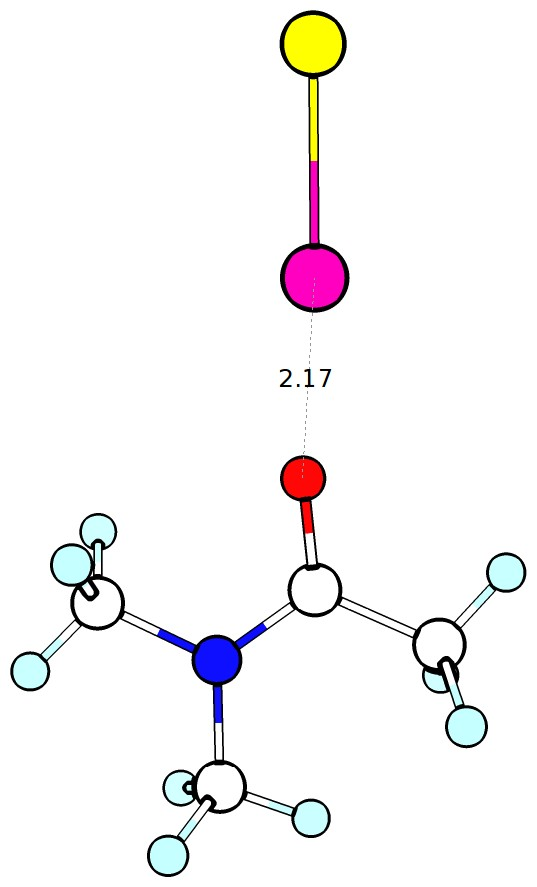
\includegraphics[width=4cm]{figures/dma-na-cl}
	}
  \subfigure[Acetyl radical]{
		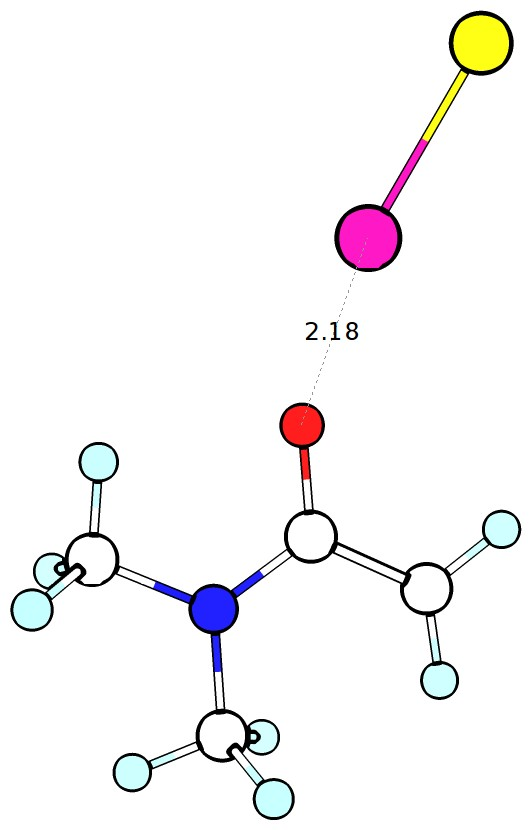
\includegraphics[width=4cm]{figures/dma-na-cl-acetyl}
	}
  \subfigure[Cis radical]{
    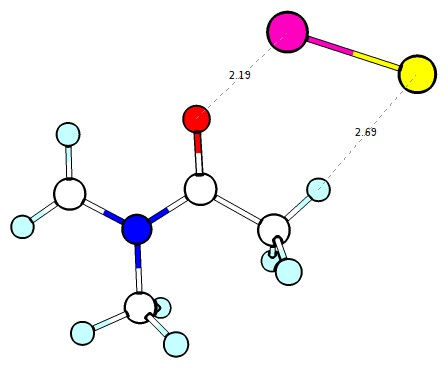
\includegraphics[width=6cm]{figures/dma-na-cl-cis}
  }
  \subfigure[Trans radical]{
    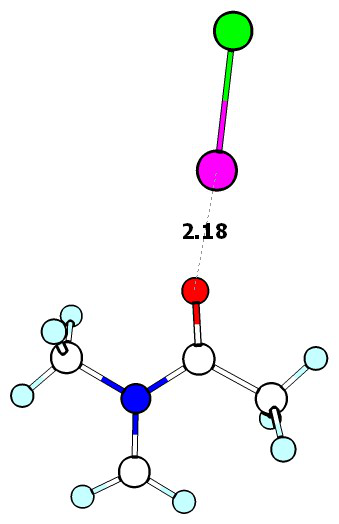
\includegraphics[width=4cm]{figures/dma-na-cl-trans}
  }

\caption[Structures of the DMA-NaCl complex and associated radical
complexes.]{Structures of \textbf{a} the DMA-NaCl complex, \textbf{b} the
DMA-NaCl acetyl radical complex, \textbf{c} the DMA-NaCl cis
radical complex, and \textbf{d} the DMA-NaCl trans radical complex. Key
interaction distances are shown in units of \AA. Element colour key: white is
carbon, light blue is hydrogen, red is oxygen, blue is nitrogen, purple is
sodium, and green is chlorine.} \label{fig:dma-na-cl}
\end{figure}

Interestingly, the predicted BDE for the acetyl radical of DMA decreases with
both \ch{Na^+} and \ch{NaCl}. This can be attributed to the change in
electronic structure associated with complexation. Consider the two possible
resonance forms of DMA shown in ~\ref{fig:dma-res}. \cite{Hrabal1997} utilized
natural resonance theory to estimate that the right-hand resonance structure in
the closely related formamide constributes about 30\% to the overall resonance
hybrid. On the other hand, straight forward NBO analysis predicts a bond order
in DMA of 1.5 between the C and O and the C and N. Nonetheless, the
complexation of DMA to \ch{Na^+} slightly increases the contribution of the
zwitterionic form, resulting in a decrease in electron density at the carbonyl
carbon. This is evidenced by the increase in NPA charge at the carbonyl from
+0.72 in DMA to +0.74 in the DMA-\ch{Na^+} complex.  The partially
positively-charged carbon centre inductively withdraws electron density,
stabilizing the acetyl radical, increasing the $\pi$ bonding character between
the two carbon centres, and decreasing the effective BDE. This is also
evindence by the decrease in the carbonyl-acetyl C-C bond lengths in the acetyl
radical, which decrease from 1.457 $\AA$ to 1.443 $\AA$ upon complexation of
\ch{Na^+}. Complexation of \ch{NaCl} results in a bond length of 1.451 $\AA$,
which is consistent with the BDE results.  On the other hand, the amidic
nitrogen becomes net more positive, but still has an NPA charge which is
negative. As a results, there is no inductive stabilization effect for the
$N$-methyl radicals.

\begin{figure}[!htpb]
  \centering
  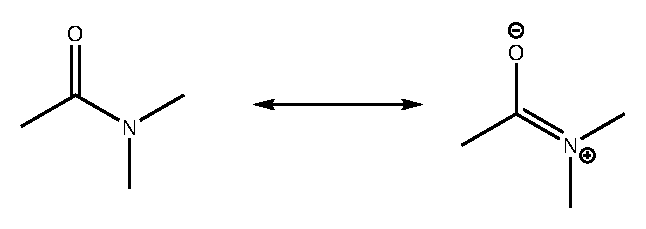
\includegraphics[width=0.7\textwidth]{figures/DMA-resonance.eps}
  \caption{The resonance forms of DMA.}
  \label{fig:dma-res}
\end{figure}

For MeCN and DMSO the complexation of either \ch{Na^+} or \ch{NaCl} results in
a decrease in \ch{C-H} BDE.\@ In MeCN, the hyperconjugative overlap between the
\ch{C+N} $\pi$-system and the \ch{C-H} $\sigma^*$ anti-bonding orbital
decreases as a result of the interaction between \ch{Na^+} and the nitrogen
centre. DMSO has a non-Lewis electronic structure, making it difficult to
analyze orbital interactions of valence-bond orbitals. Nonetheless, there is
normally a nominal hyperconjugative overlap between the sulphur centre and the
\ch{C-H} $\sigma^*$ anti-bonding orbitals, which was confirmed by NBO analysis.
This overlap decreases as a result of the interaction of \ch{Na^+} with the
oxygen-centre of DMSO.

Upon complexation of \ch{Na+} of \ch{NaCl}, the BDEs of the more sterically
bulky amide substrate DIA follow the same trend that is observed as for DMA:
The acetyl \ch{C-H} BDE decreases due to inductive stabilization, while the
\ch{C-H} bonds $\alpha$ to the amidic nitrogen centre increase as a result of
decreased hyperconjugative overlap. Alkoxyl radicals are not expected to
abstract from \ch{C-H} bonds $\beta$ to the nitrogen centre in DIA or other
longer chain $N$-alkyl amides, as the incipient radical is not stabilized by
amidic $\pi$-system. However, that due to steric repulsion, the
$\alpha$-radicals of DIA cannot lie directly in the $\pi$-plane. As such the
$\alpha$-\ch{C-H} BDEs of DIA are greater than those of DMA by 2-3 \kcalmol,
and are closer to the $\beta$-\ch{C-H} BDEs than perhaps expected. The effects
of sodium binding to the amidic oxygen are almost nil for the $\beta$-trans C-H
bond of DIA, however there is a significant decrease in the $\beta$-cis
\ch{C-H} BDE.  \ref{fig:dia-na-cl}a,b shows the structures of the DIA-NaCl
complex and the $\beta$-cis radical complex, where it can seen that the metal
cation interacts with both the oxygen-centre and the carbon-centred radical.
This interaction stabilizes the radical complex and thus decrease the effective
BDE, however this interaction is likely not possible in the TS structure and is
not expected to contribute to the effective BDE in a HAT reaction.

\begin{figure}[!htbp]
	\centering

	\subfigure[DIA-NaCl]{
		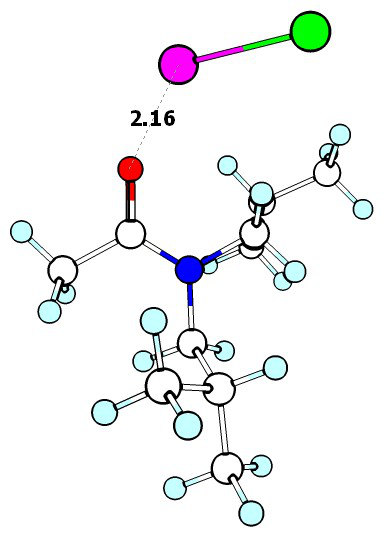
\includegraphics[width=4cm]{figures/dia-na-cl}
	}
  \subfigure[$\beta$-cis radical]{
		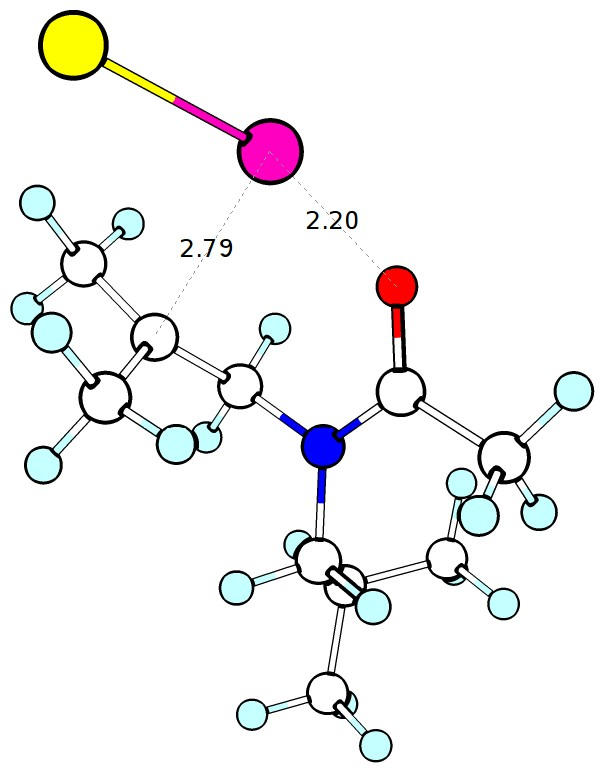
\includegraphics[width=4cm]{figures/dia-na-cl-rad-b}
	}

  \caption[Structures of the DIA-NaCl complex and radical complex.]{Structures
  of \textbf{a} the DMA-NaCl complex, \textbf{b} the DIA-NaCl $\beta$-cis
  radical complex. Key interaction distances are shown in units of \AA. Element
  colour key: white is carbon, light blue is hydrogen, red is oxygen, blue is
  nitrogen, purple is sodium, and green is chlorine.} \label{fig:dia-na-cl}
\end{figure}

All of these results together confirm that specific metal-substrate
interactions can increase the effective BDEs of abstractable \ch{C-H} bonds by
decreasing hyperconjugative overlap. However, this is complicated by the
possibility for secondary interactions between the metal or counter-anion.
Furthermore, additional factors such as induction can alter the effects. It
appears that for \ch{C-H} bonds $\alpha$ to electron-rich species which
hyperconjugatively overlap with the $\sigma^*$ anti-bonding orbital, the
complexation of non-redox active metals increases the effective \ch{C-H} bond
strength. However, if the \ch{C-H} bond is adjacent to an electron-poor centre,
such as the carbon of a carbonyl, metal complexation actually decreases the
bond strength slightly. In the context of HAT reaction barrier heights,
increasing the effective \ch{C-H} bond strength should decrease the
reaction-rate slightly by destabilizing the TS complex. However, there are
other important factors to consider such as polarity in the TS complex.
Furthermore, it is important to note that experiments showed that \ch{NaClO4}
did not significantly effect the HAT rate constants for reactions between
\cumo\ and organic substrates. Therefore, the effects observed herein likely
are an exaggeration of what is truly occurring in situ. Nonetheless, these
theoretical calculations may be useful in developing an understanding of the
subtle nature of the effects of non-redox active metal cations on HAT reactions
in general.

\section{HAT reactions involving non-redox active metals}

\subsection{DMA}

Hydrogen abstraction reactions involving the oxygen-centred radicals \bno\ and
\cumo\ and DMA in MeCN have been previously investigated experimentally and
theoretically.\cite{Salamone2013} The HAT reaction between DMA and \bno\ was
determined to occur dominantly through a direct HAT mechanism from the
$N$-methyl group cis relative to the carbonyl, and is kinetically limited by
the formation of a strong pre-reaction complex between the relatively acid
$\alpha$-C-H of \bno\ and the amidic oxygen centre. On the other hand, \cumo\
cannot form a strong hydrogen-bonding interaction, and thus can form a
non-specific dispersion-bound pre-reaction complexes. Abstraction by \cumo\
still takes place from one of the $N$-methyl groups, but the rate constant is 2
orders of magnitude less than for \bno. Recall that the inclusion of metal
salts in reactions of DMA with \cumo\ were previously
investigated.\cite{Salamone2015metals} On the basis of the exaggerated effects
observed in the changes in BDEs and the technical difficulties associated with
these studies, the goal of this work is not to reproduce experimental results,
but rather, develop insights into the possible changes that can occur as a
result of metal salt addition to HAT reactions.

Herein, I have calculated the reaction barrier heights for all three
abstractable positions of DMA for HAT reactions involving \cumo\ and \bno, both
with and without \ch{NaCl}. These data are summarized in~\ref{tab:DMA-dG}. The
free energy barriers calculated at the
M05-2X-SMD(MeCN)/6-311+G(2d,2p)//M05-2X/6-31+G$^{**}$ are systematically higher
than those previously calculated by about 8.5 \kcalmol.\cite{Salamone2013} The
reason for this is unclear, given that M05-2X has previously been used
successfully to calculate accurate HAT rate constants.\cite{Galano2013}
However, the relative ranking and differences energies for the reaction barrier
heights for the different \ch{C-H} bonds are consistent with previous results.
Therefore, although these results cannot be used to predict rate constants,
they are useful for studying the change in barrier height due to the addition
of NaCl.

\begin{table}[!htbp]
\caption[Calculated free energy (enthalpy) barrier for direct HAT from
different \ch{C-H} bonds in DMA by \cumo\ and \bno, with and without
\ch{NaCl}.]{Calculated free energy (enthalpy) barrier ($\Delta G(H)^\ddagger$,
\kcalmol) for direct HAT from different \ch{C-H} bonds in DMA by \cumo\ and
\bno, with and without \ch{NaCl}. The change in barrier height is calculated
relative to the same abstraction site without the inclusion of \ch{NaCl}. All
barrier heights are relative to separated reactants and were calculated at the
M05-2X-SMD(MeCN)/6-311+G(2d,2p)//M05-2X/6-31+G$^{**}$ level of theory.}
\label{tab:DMA-dG}
  \begin{tabular}{l l c c}
Reaction   & Abstraction Site &  $\Delta G(H)^\ddagger$ & $\Delta\Delta G(H)^\ddagger$ \\
\hline
DMA + \cumo   &  trans              &  17.3(3.4)           &              \\
              &  cis                &  17.5(3.8)           &              \\
              &  acetyl             &  21.6(7.5)           &              \\
DMA-NaCl + \cumo &  trans              &  20.3(3.7)        &    3.0(0.3)  \\
              &  cis                &  18.4(1.2)           &    0.9(-2.6) \\
              &  acetyl             &  21.0(4.3)           &   -0.6(-3.2) \\
DMA + \bno    &  trans              &  16.5(3.7)           &              \\
              &  cis                &  17.5(3.6)           &              \\
              &  acetyl             &  20.8(7.8)           &              \\
DMA-NaCl + \bno &  trans              &  18.6(1.7)         &    2.1(-2.0) \\
              &  cis                &  17.8(4.7)           &    0.3(1.1)  \\
              &  acetyl             &  22.0(4.7)           &    1.2(-3.1)
  \end{tabular}
\end{table}

Focussing first on the barrier heights for HAT between DMA and \cumo, the
results of complexation with \ch{NaCl} is variable. For each of the acetyl,
cis, and trans \ch{C-H} bond positions of DMA, there are three different
effects upon complexation of \ch{NaCl}. For the trans position, both the free
energy and enthalpic barriers increase, for the cis position the free energy
barrier increases and the enthalpic barrier decreases, and for the acetyl
position both the free energy and enthalpic barriers decrease. The reason for
this relies on examining the TS structures, which are shown
in~\ref{fig:dma-cumo-ts}a-f.

\begin{figure}[!htbp]
  \centering

  \subfigure[Trans DMA + \cumo]{
		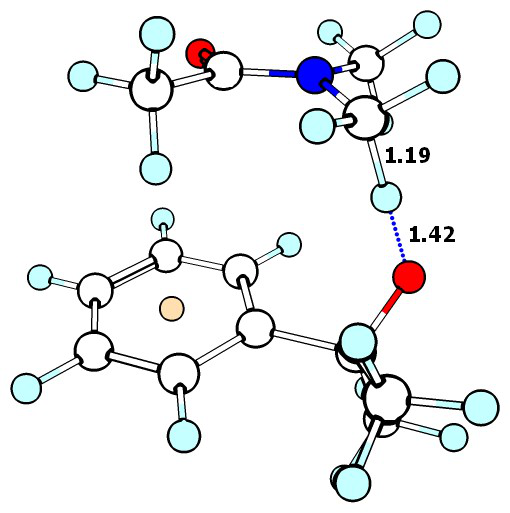
\includegraphics[width=4cm]{figures/dma-cumo-trans}
	}
  \subfigure[Trans DMA-NaCl + \cumo]{
		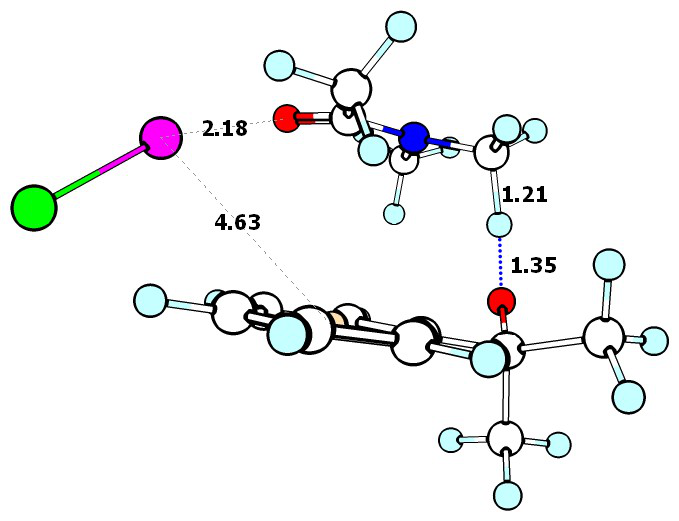
\includegraphics[width=4cm]{figures/dma-nacl-cumo-trans}
	}

  \subfigure[Cis DMA + \cumo]{
    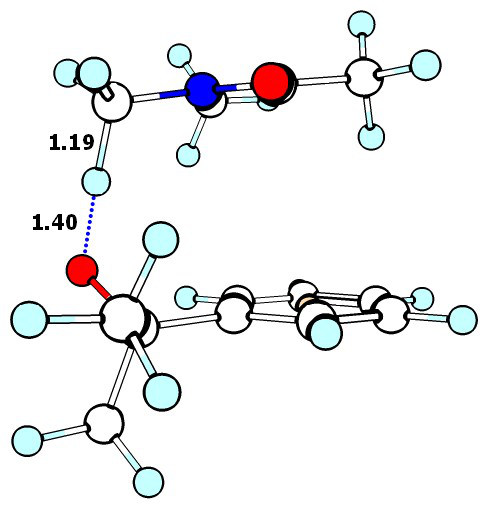
\includegraphics[width=4cm]{figures/dma-cumo-cis}
  }
  \subfigure[Cis DMA-NaCl + \cumo]{
		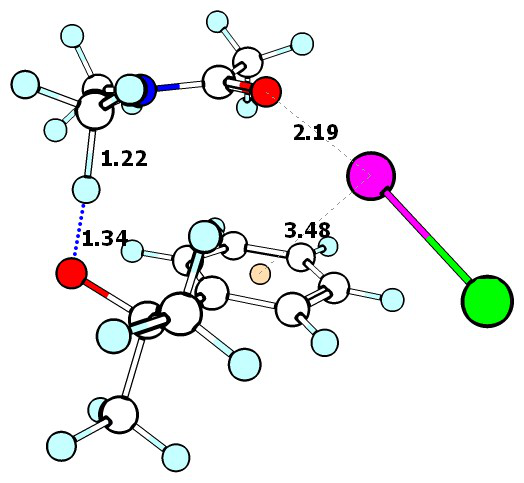
\includegraphics[width=4cm]{figures/dma-nacl-cumo-cis}
	}
  \caption{}
\end{figure}

\begin{figure}[!htbp]\ContinuedFloat
  \subfigure[Acetyl DMA + \cumo]{
    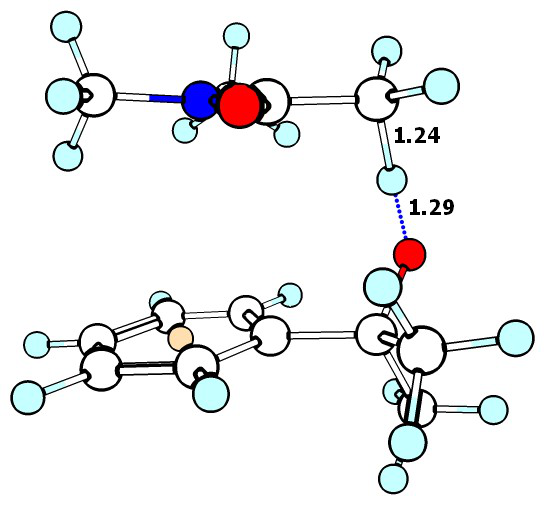
\includegraphics[width=4cm]{figures/dma-cumo-acetyl}
  }
  \subfigure[Acetyl DMA-NaCl + \cumo]{
    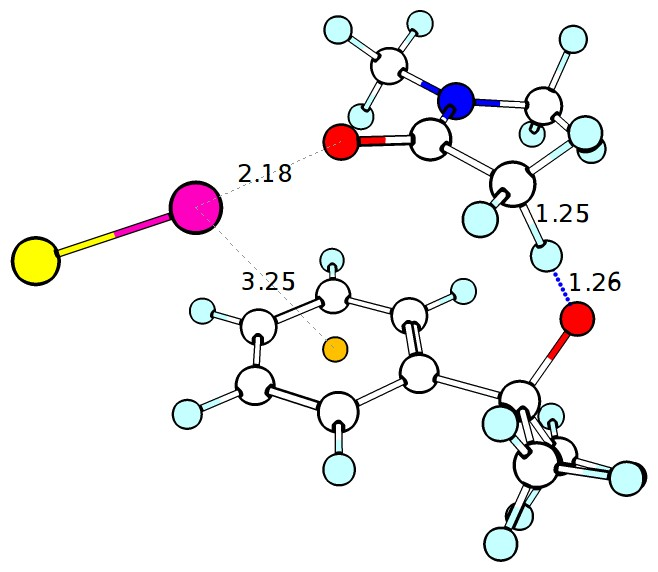
\includegraphics[width=4cm]{figures/dma-nacl-cumo-acetyl}
  }

  \caption[TS structures of HAT reaction between DMA and \cumo\ including and
  excluding NaCl.]{TS structures of HAT reaction between DMA and \cumo\
  including NaCl for different \ch{C-H} bonds: \textbf{a} trans, \textbf{b}
  trans with NaCl, \textbf{c} cis, \textbf{d} cis with NaCl, \textbf{e} acetyl,
  and \textbf{f} acetyl with NaCl. Key interatomic distances are shown in units
  of \AA. Element colour key: white is carbon, light blue is hydrogen, red is
  oxygen, blue is nitrogen, purple is sodium, green is chlorine, and peach is a
  dummy atom in the centre of an aromatic ring.} \label{fig:dma-cumo-ts}
\end{figure}

For the TS structure representing abstraction from the trans position (relative
to the carbonyl) \ch{C-H} bond of DMA by \cumo\ (\ref{fig:dma-cumo-ts}a), there
is a calculated 0.3 \kcalmol\ increase in $\Delta H^\ddagger$, which is
somewhat less than the predicted increase in BDE of 1.0 \kcalmol. This
difference can be ascribed as due to the effect of charge transfer: NPA
indicates a 0.04 $e^-$ transfer from DMA to \ch{Na^+}. Furthermore, TSs for HAT
between \ch{C-H} bond and oxygen-centred radicals are characterized by a degree
of charge separation.\cite{Roberts1999} NPA indicates that in the trans
position TS structure excluding \ch{NaCl} the charge separation is 0.24 $e^-$,
but the charge separation increases with the inclusion of \ch{NaCl} to 0.26
$e^-$. This increased charge separation results in a lower enthalpic barrier
than expected solely on the basis of the increase in \ch{C-H} BDE. By
increasing charge separation in the TS structure, it becomes easier to abstract
the hydrogen atom as it increases the proton-transfer like character. The
increase in $\Delta G^\ddagger$ is 3.0 \kcalmol, therefore the complexation of
metal cations increases the entropic penalty in forming the TS structure, or in
other words the TS is tighter than in the absence of metal cations.

In abstraction of the cis position \ch{C-H} bond of DMA by \cumo, there is a
calculated 2.6 \kcalmol\ decrease in $\Delta H^\ddagger$ and an increase of 0.9
\kcalmol\ in $\Delta G^\ddagger$. The decrease in enthalpic barrier is
inconsistent with the predicted increase in BDE of 1.8 \kcalmol\ upon
complexation with \ch{NaCl}. The TS structure in~\ref{fig:dma-cumo-ts}c shows a
possible long range interaction between \ch{Na^+} and the aromatic ring of
\cumo which draws electron density and increases the reactivity. Additionally,
NPA predicts a 0.07 $e^-$ charge transfer between DMA and \ch{Na^+}. The
combination of these two factors stabilizes the TS and decreases $\Delta
H^\ddagger$. The entropic penalty associated with complexation of \ch{NaCl}
results in an increase in free energy barrier.

Abstraction by \cumo\ from the acetyl \ch{C-H} bond of DMA was previously
described as being a minor reaction pathway.\cite{Salamone2013} In light of the
reduction in BDE at the acetyl position of amides, it may be reasonable to
expect the reaction barrier to decrease. This indeed appears to be the net
effect of complexation of \ch{NaCl} to DMA, as $\Delta H^\ddagger$ decreases by
3.1 \kcalmol\ and $\Delta G^\ddagger$ decreases by 0.6 \kcalmol.
\ref{fig:dma-cumo-ts}f shows that in the TS structure, \ch{Na^+} interacts with
the aromatic system of \cumo, which also stabilizes the TS and decreases the
barrier.

For HAT between DMA and \bno, the interaction between \ch{NaCl} and \bno, are
stronger owing to the shorter distance between \ch{Na^+} and the centre of the
aromatic ring, as shown in~\ref{fig:dma-bno-ts}a-f. This shorter distance is
likely possible due to the easier rotation of DMA relative to \bno, as compared
to \cumo. As a result, the enthalpic barriers for the abstraction from DMA by
\bno\ decrease as a result of complexation of \ch{NaCl} for both the acetyl and
trans position \ch{C-H} bonds. For the cis position \ch{C-H} bond of DMA
however, the enthalpic barrier increases. This can be explained on the basis of
the presence of an interaction between \ch{Cl^-} and the $\alpha$\ch{C-H} bond
of \bno. While \ch{Na^+} withdraws electron density from the aromatic system of
\bno, \ch{Cl^-} is able to donate electron density back to \bno, counteracting
the effect of the interaction of \ch{Na^+}. As a result, the enthalpic barrier
increases as predicted on the basis of the increase of the cis position
\ch{C-H} BDE of DMA.

\begin{figure}[!htbp]
  \centering

  \subfigure[Trans DMA + \bno]{
		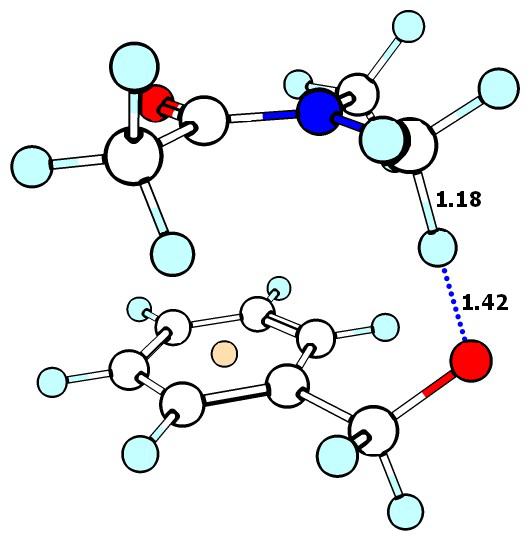
\includegraphics[width=4cm]{figures/dma-bno-trans}
	}
  \subfigure[Trans DMA-NaCl + \bno]{
		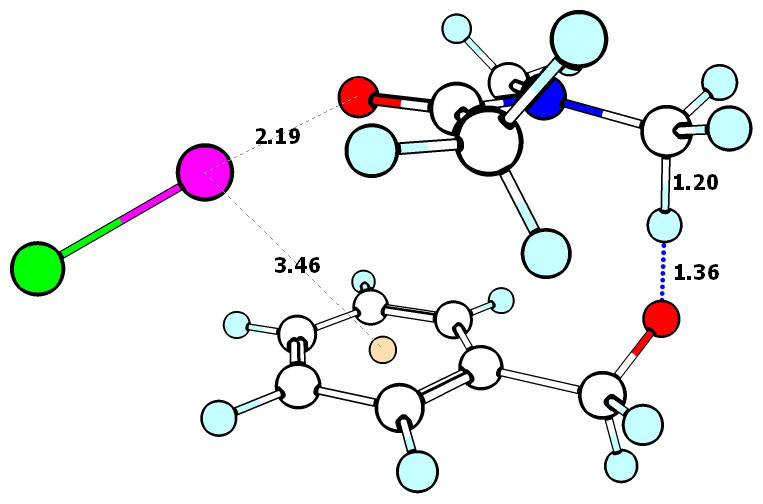
\includegraphics[width=4cm]{figures/dma-nacl-bno-trans}
	}

  \subfigure[Cis DMA+ \bno]{
		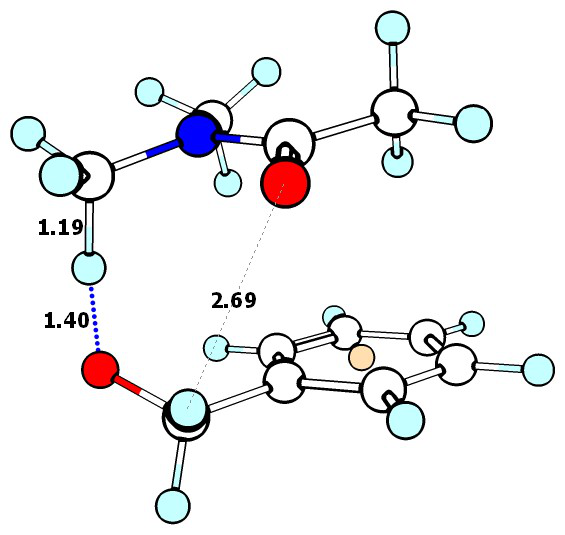
\includegraphics[width=4cm]{figures/dma-bno-cis}
	}
  \subfigure[Cis DMA-NaCl + \bno]{
		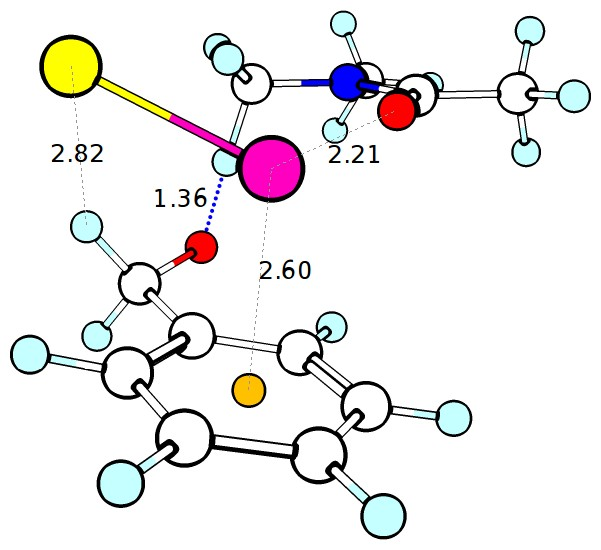
\includegraphics[width=4cm]{figures/dma-nacl-bno-cis}
	}
  \caption{}
\end{figure}

\begin{figure}[!htbp]\ContinuedFloat
  \subfigure[Acetyl DMA + \bno]{
    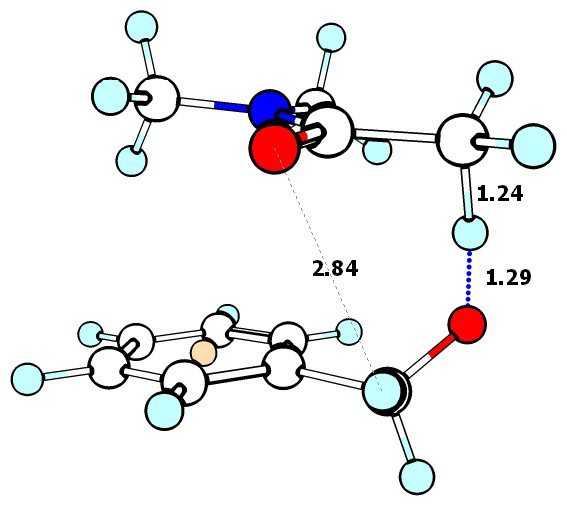
\includegraphics[width=4cm]{figures/dma-bno-acetyl}
  }
  \subfigure[Acetyl DMA-NaCl + \bno]{
    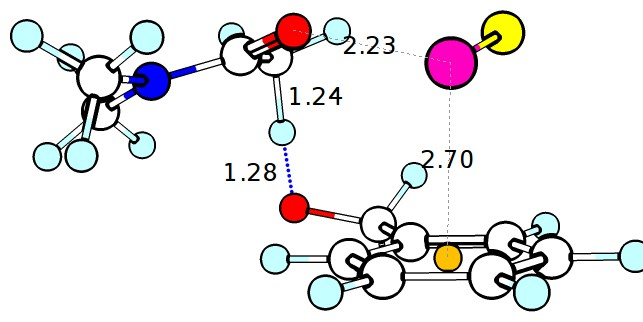
\includegraphics[width=4cm]{figures/dma-nacl-bno-acetyl}
  }

  \caption[TS structures of HAT reaction between DMA and \bno\ including
  NaCl.]{TS structures of HAT reaction between DMA and \bno\ including NaCl for
  different \ch{C-H} bonds: \textbf{a} trans, \textbf{b} trans with NaCl,
  \textbf{c} cis, \textbf{d} cis with NaCl, \textbf{e} acetyl, and \textbf{f}
  acetyl with NaCl. Key interatomic distances are shown in units of \AA.
  Element colour key: white is carbon, light blue is hydrogen, red is oxygen,
  blue is nitrogen, purple is sodium, green is chlorine, and peach is a dummy
  atom in the centre of an aromatic ring.} \label{fig:dma-bno-ts}
\end{figure}

For both \cumo\ and \bno, the presence of possible secondary interactions
between \ch{NaCl} and the radicals obfuscates the results. Therefore, in order
to determine if non-redox active metal cations may act as chemo-protective
agents in biological systems, I have performed calculated involving the more
biologically relevant \ch{HO^.} radical. Although there is no literature value
for $k_H$ of the HAT reaction between DMA and \ch{HO^.}, I have used the
Snelgrove-Ingold equation\cite{Snelgrove2001} to estimate the rate constant as
1.5\E{10} \Ms, which is two and five orders of magnitude greater than \bno\ and
\cumo, respectively. Unfortunately, I was unsuccessful in performing full
optimization calculations in the presence of the metal salt. However, the
``guess'' TS structures obtained by freezing the hydrogen atom acceptor donor
bonds (as described in the methods section) herein represent approximated
transition state structures and therefore provide an estimate of the effects of
metal salts in a more biologically relevant model. The calculated reaction
barriers are presented in~\ref{tab:dma-oh}.

\begin{table}[!htbp]
\caption[Calculated free energy (enthalpy) barrier for direct HAT from
different \ch{C-H} bonds in DMA by \ch{HO^.}, with and without
\ch{NaCl}.]{Calculated free energy (enthalpy) barrier ($\Delta G(H)^\ddagger$,
\kcalmol) for direct HAT from different \ch{C-H} bonds in DMA by \ch{HO^.},
with and without \ch{NaCl}. The change in barrier height is calculated relative
to the same abstraction site without the inclusion of \ch{NaCl}. All barrier
heights are relative to separated reactants and were calculated at the
M05-2X-SMD(MeCN)/6-311+G(2d,2p)//M05-2X/6-31+G$^{**}$ level of theory.
$^*$Indicates estimated barrier based on ``guess'' TS structure.}
\label{tab:dma-oh}
  \begin{tabular}{l l c c}
Reaction   & Abstraction Site &  $\Delta G(H)^\ddagger$ & $\Delta\Delta G(H)^\ddagger$ \\
\hline
DMA + \ch{HO^.} &  trans           &  8.9(0.0)            &                \\
            &  cis                &  7.9(-2.7)           &                    \\
            &  acetyl             &  9.9(0.5)            &                    \\
DMA-NaCl + \ch{HO^.}&  trans$^*$      &  13.1(1.3)           &  4.2(1.3)          \\
            &  cis$^*$                &  12.9(0.2)           &  5.0(2.9)          \\
            &  acetyl$^*$             &  16.6(2.0)           &  7.7(1.5)          \\
  \end{tabular}
\end{table}

For the direct HAT reaction between \ch{OH^.} and DMA abstraction occurs
primarily from the cis position \ch{C-H} bond of DMA. The calculated free
energy (enthalpic) barrier is 7.9(-2.7) \kcalmol, which gives a calculated rate
constant of 1.0 \E{7} \Ms, or three orders of magnitude lower than the
predicted rate constants of 1.5 \E{10} \Ms. This result in unsurprising given
the poor agreement of HAT reaction between DMA and \bno\ and \cumo. For
abstraction by \ch{HO^.}, the complexation of \ch{NaCl} to DMA increases the
estimated free energy reaction barriers across the board by 4.2--7.7 \kcalmol.
This suggests that if \ch{Na^+} interacts closely with DMA in vivo, then
non-redox active metals may have a chemo-protective effect against hydrogen
abstraction by \ch{HO^.}.

For the acetyl position \ch{C-H} bond of DMA, the enthalpic barrier increases
by 1.5 \kcalmol, even though the calculated BDE decreases slightly upon
complexation of \ch{NaCl}. This can once again be explained by the effects of
charge transfer in the TS complex. For the TS structure representing direct HAT
between \ch{HO^.} the acetyl position of DMA-NaCl, there is a calculated charge
transfer from DMA to \ch{Na^+} of 0.02 $e^-$, which results in a decrease in
charge separation between \ch{HO^.} and DMA from 0.26 $e^-$ without \ch{NaCl}
to 0.25 $e^-$ with \ch{NaCl}. Although this effect is small, it appears to
significantly effect the ability of \ch{HO^.} to abstract a hydrogen atom from
DMA. The same argument applies to both the cis and trans \ch{C-H} bond
positions of DMA, for which the enthalpic barrier increases by more than the
calculated change in BDE. For the significantly more reactive \ch{HO^.}
radical, the metal is less likely to interact with the oxygen centre, thus the
effects observed depend only on interactions with DMA. As a result, the
reaction barrier increases in all cases upon complexation of \ch{NaCl}.

\subsection{DIA}

Next, to study the effect steric bulk has on the HAT reactions between amides
and oxygen-centred radical, I have performed a study of HAT between DIA and
\cumo. The HAT reaction between DIA and \cumo\ was previously studied by
\citet{Salamone2014}, however only the $\alpha$-N-alkyl positions were studied
theoretically. Since the BDEs for $\alpha$- and $\beta$-N-alkyl \ch{C-H}
positions are relatively close in energy, I calculated the reaction barriers
for these positions as well. The calculated free energy (enthalpic) barriers
excluding and including \ch{NaCl} are listed in ~\ref{tab:dia-cumo}.
Interestingly the predicted reaction barriers for abstraction of the
$\beta$-positions of DIA are lower than the $\alpha$-positions. By applying the
Boltzmann distribution about 69\% of abstractions by \cumo\ from DIA will take
place from either the cis- or trans-$\beta$ positions of DIA. Therefore,
abstraction from bulky amides by bulky oxygen-centred radicals are likely
controlled by steric considerations. Note also that many of the TS
optimizations were not successful with the inclusion of \ch{NaCl} and in which
case ``guess'' TS structures have been used to estimate the barrier heights.
The TS structures for the HAT reaction between DIA and \cumo\ including
\ch{NaCl} are shown in~\ref{fig:dia-cumo-ts}.

\begin{table}[!htbp]
\caption[Calculated free energy (enthalpy) for direct HAT from different
\ch{C-H} bonds in DIA by \cumo, with and without \ch{NaCl}.]{Calculated free
energy (enthalpy) ($\Delta G(H)^\ddagger$, \kcalmol) for direct HAT from
different \ch{C-H} bonds in DIA by \cumo, with and without \ch{NaCl}. The
change in barrier height is calculated relative to the same abstraction site
without the inclusion of \ch{NaCl}. All barrier heights are relative to
separated reactants and were calculated at the
M05-2X-SMD(MeCN)/6-311+G(2d,2p)//M05-2X/6-31+G$^{**}$ level of theory.
$^*$Indicates estimated barrier based on ``guess'' TS structure.}
\label{tab:dia-cumo}
  \begin{tabular}{l l c c}
    Reaction   &  Abstraction Site   &  $\Delta G(H)^\ddagger$ &  $\Delta \Delta G(H)^\ddagger$ \\
    \hline
    DIA + \cumo    &  $\alpha$-trans    &  19.5(6.2)  &              \\
                   &  $\alpha$-cis      &  19.1(5.4)  &              \\
                   &  $\beta$-trans     &  18.6(6.0)  &              \\
                   &  $\beta$-cis       &  18.4(6.5)  &              \\
                   &  acetyl         &  19.1(7.4)  &              \\
    DIA-NaCl + \cumo &  $\alpha$-trans$^*$  &  17.0(3.9)  &   -2.5(-2.3)  \\
                   &  $\alpha$-cis$^*$      &  12.7(-2.4) &   -6.4(-7.8) \\
                   &  $\beta$-trans     &  19.8(6.8)  &    0.7(1.4)  \\
                   &  $\beta$-trans$^*$     &  19.6(6.9)  &    0.5(1.5)  \\
                   &  $\beta$-cis$^*$       &  16.8(4.2)  &   -1.6(-2.3) \\
                   &  acetyl$^*$         &  17.8(3.8)  &    0.8(-0.1) \\
                   &  acetyl             &  17.9(3.7)  &    0.9(-0.2)
  \end{tabular}
\end{table}

\begin{figure}
  \centering

  \subfigure[$\alpha-$trans DIA-NaCl + \cumo]{
		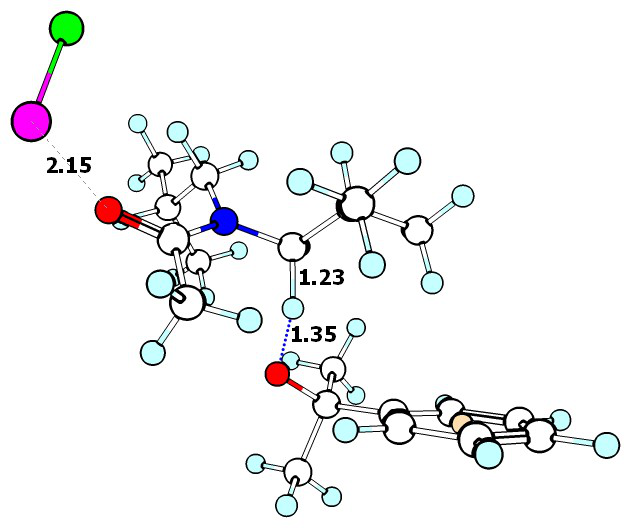
\includegraphics[width=4cm]{figures/dia-nacl-cumo-trans-alpha}
	}
  \subfigure[$\alpha-$cis DIA-NaCl + \cumo]{
		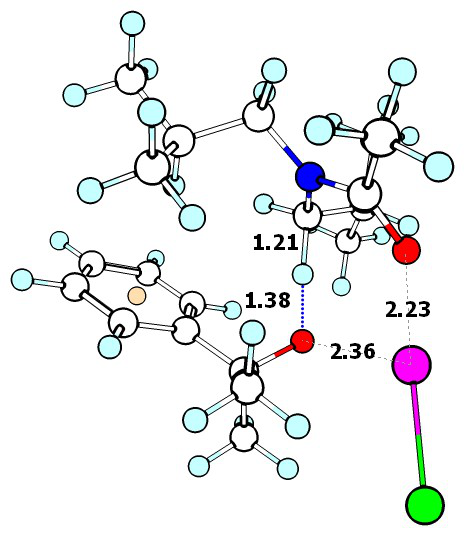
\includegraphics[width=4cm]{figures/dia-nacl-cumo-cis-alpha}
	}

  \subfigure[$\beta-$trans DIA-NaCl + \cumo]{
		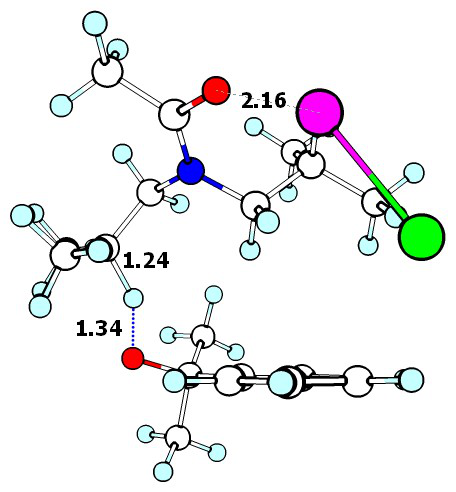
\includegraphics[width=4cm]{figures/dia-nacl-cumo-trans-beta}
	}
  \subfigure[$\beta-$cis DIA-NaCl + \cumo]{
		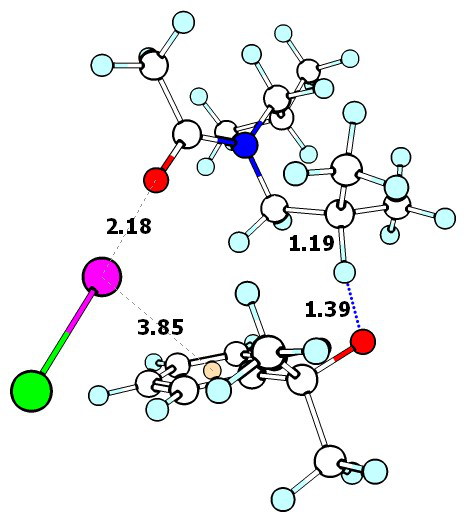
\includegraphics[width=5cm]{figures/dia-nacl-cumo-cis-beta}
	}
  \caption{}
\end{figure}

\begin{figure}\ContinuedFloat
  \subfigure[Acetyl DIA-NaCl + \cumo]{
    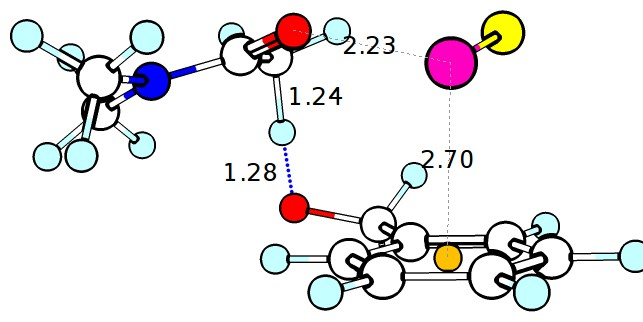
\includegraphics[width=5cm]{figures/dma-nacl-bno-acetyl}
  }

  \caption[TS structures for HAT reaction between DIA and \cumo\ including
  NaCl.]{TS structures for HAT reactions between DIA and \cumo\ including NaCl
  for different \ch{C-H} bonds: \textbf{a} $\alpha$-trans, \textbf{b}
  $\alpha$-cis, \textbf{c} $\beta$-trans, \textbf{d} $\beta$-cis, and
  \textbf{e} acetyl. Key interatomic distances are shown in units of \AA.
  Element colour key: white is carbon, light blue is hydrogen, red is oxygen,
  blue is nitrogen, purple is sodium, green is chlorine, and peach is a dummy
  atom in the centre of an aromatic ring.} \label{fig:dia-cumo-ts}
\end{figure}

As was observed in the barrier height calculations involving \ch{NaCl} with DMA
with \bno\ and \cumo, the results vary depending on the presence or absence of
secondary interactions of \ch{Na^+} with \cumo. For the $\beta$-cis and acetyl
position of DIA (\ref{fig:dia-cumo-ts}d-e), $\Delta H^\ddagger$ decreases by
2.3 and 0.2 \kcalmol, respectively, as a result of relatively long range
interactions of \ch{Na^+} with the aromatic system of \cumo. For abstraction
from the $\alpha$-cis position of DIA (\ref{fig:dia-cumo-ts}b), \ch{Na^+} is
able to interact with both the amidic oxygen lone pair, and a lone pair on the
oxygen of \cumo, resulting in a significant decrease in $\Delta H^\ddagger$ by
7.8 \kcalmol.

For the $\alpha$-trans position there is no interaction between \ch{Na^+} and
\cumo, however the complexation of \ch{Na^+} to DIA results in a 2.5 \kcalmol\
decrease in $\Delta G^\ddagger$. Comparing the TS structures including and
excluding NaCl, there is very little difference. Therefore, it is likely that
the ``guess'' TS structure including NaCl does not appropriately represent the
``true'' TS structure for this particular abstraction site. Note that this may
also be the case in other systems.

Abstraction by \cumo\ from the $\beta$-trans position of DIA does not allow for
an interaction between both the amidic oxygen and \cumo. However, there should
be no effect from decreasing hyper Consequently, $\Delta H^\ddagger$ increases
by 1.4 \kcalmol\ as a result of the effect of 0.04 $e^-$ charge transfer from
DIA to \ch{Na^+} in the TS structure.


\subsection{Strong hydrogen bond accepting substates}

In the investigation of the effects of metal cations on HAT reactions between
DMA and \cumo\ Salamone et al. demonstrated that in DMSO solvent, HAT
reactivity is not significantly effected by the addition of metal
salts.\cite{Salamone2015metals} This can be explained on the basis of the
stronger Lewis basicity of DMSO as as compared to DMA, resulting in the
competitive binding of \ch{M^n+} to DMSO over DMA. The rate constant for HAT
between DMSO and \cumo\ is 1.8 \E{4} \Ms\ while that for DMSO and \cumo\ is 1.2
\E{6} \Ms\ in MeCN solvent at 298 K, therefore only small changes in $k_{obs}$
are expected for HAT between \cumo\ and DMA in DMSO solvent with metal salts. I
am interested in how metal salts effect the HAT reactivity of DMSO and other
related strong hydrogen bond accepting substrates. We previously showed that
DMSO and \bno\ react via an ``alternative'' HAT reaction, where \bno\ acts at
the hydrogen atom donor rather than acceptor. The net reaction yields
benzaldehyde, dimethyl sulfide, and \ch{HO^.} as the DMSO-H radical decomposes
in a concerted manner following the alternative HAT TS. \cumo\ lacks the acidic
$\alpha$-\ch{C-H} bond to donate, and therefore can only undergo conventional
HAT. I performed computational studies to determined if metal cations could
effect this reactivity and if the related (HMPA and TBPO) substrates displayed
similar reactivity.

\begin{scheme}[!htbp]
  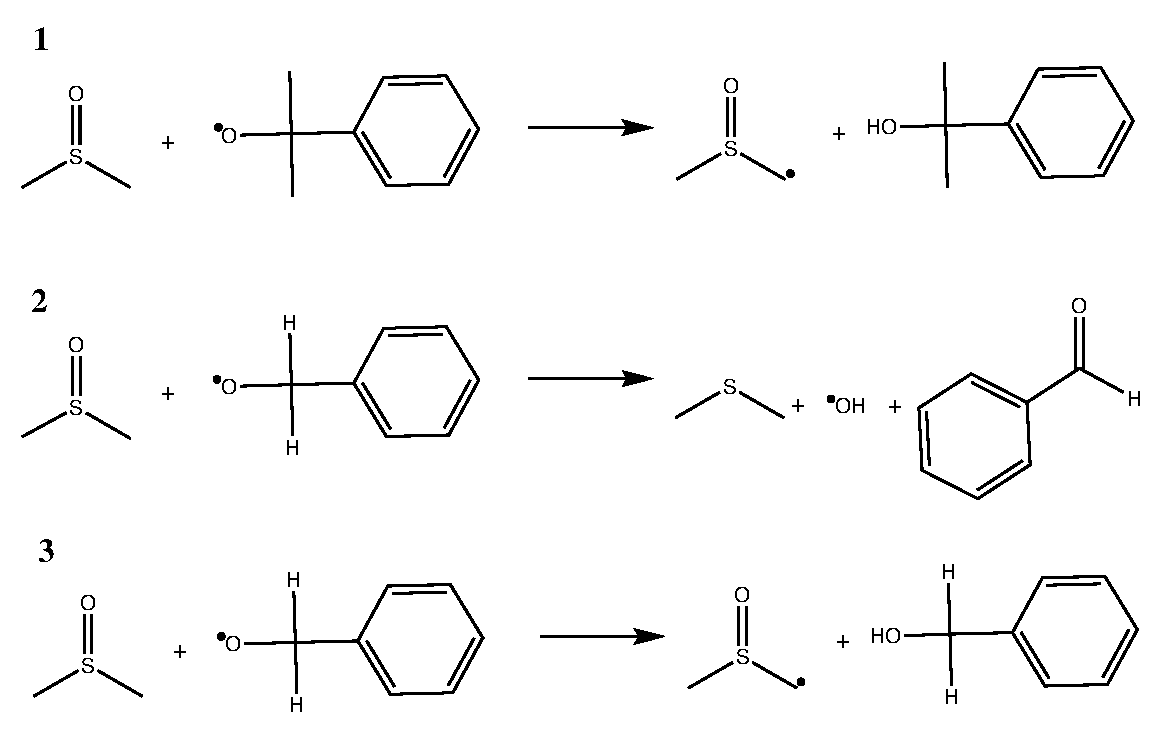
\includegraphics[width=\textwidth]{figures/dmso-rxn.eps}
  \caption[The HAT reactions of DMSO with \cumo\ and \bno.]{The HAT reactions
  of DMSO with \textbf{1} \cumo, \textbf{2} the ``alternative'' HAT reaction
  with \bno, and \textbf{3} the conventional HAT reaction with \bno.}
  \label{fig:dmso-rxn}
\end{scheme}

\begin{table}[!htbp]
\caption[Calculated free energy (enthalpy) barrier for HAT between DMSO and
\cumo, and conventional and alternative HAT with \bno, with and without
\ch{NaCl}.]{Calculated free energy (enthalpy) barrier ($\Delta G(H)^\ddagger$,
\kcalmol) for HAT between DMSO and \cumo, and conventional and alternative HAT
with \bno, with and without \ch{NaCl}. The change in barrier height is
calculated relative to the same reaction without the inclusion of \ch{NaCl}.
All barrier heights are relative to separated reactants and were calculated at
the M05-2X-SMD(MeCN)/6-311+G(2d,2p)//M05-2X/6-31+G$^{**}$ level of theory.}
\label{tab:dmso-dG}
\begin{tabular}{l c c}
Reaction    &  $\Delta G(H)^\ddagger$ &  $\Delta \Delta G(H)^\ddagger$ \\
\hline
\textbf{1}  & 20.9(8.9)  &              \\
\textbf{1} + NaCl & 22.4(5.2)  &  1.5(-3.7)   \\
\textbf{2}    & 10.4(-2.2) &              \\
\textbf{2} + NaCl & 13.4(-3.4) &  2.0(-1.2) \\
\textbf{3} & 22.7(10.4) &                  \\
\textbf{3} + NaCl & 22.1(5.2) & -0.6(-5.2)
\end{tabular}
\end{table}

\begin{figure}[!htbp]
  \centering
  \subfigure[DMSO + \cumo]{
		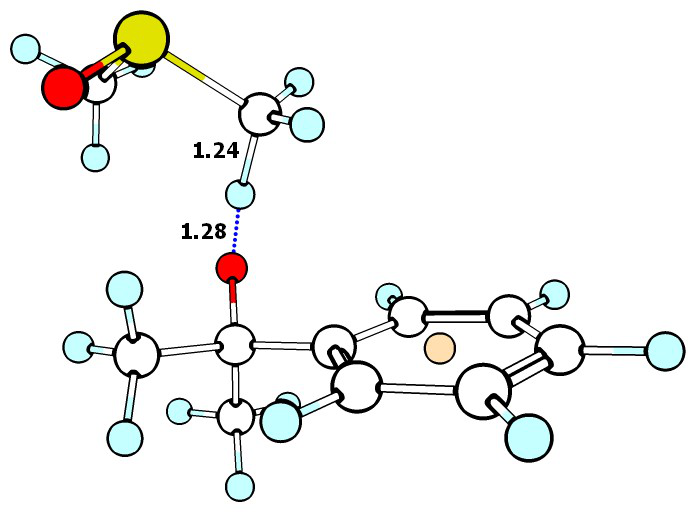
\includegraphics[width=4cm]{figures/dmso-cumo}
	}
  \subfigure[DMSO-NaCl + \cumo]{
		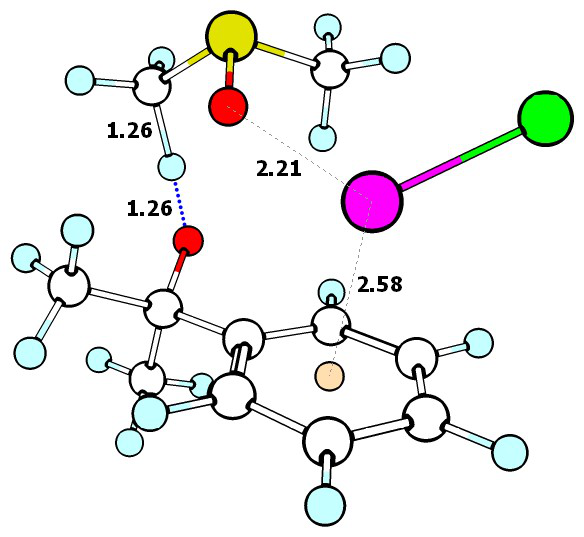
\includegraphics[width=4cm]{figures/dmso-nacl-cumo}
	}

  \subfigure[Alternative DMSO + \bno]{
    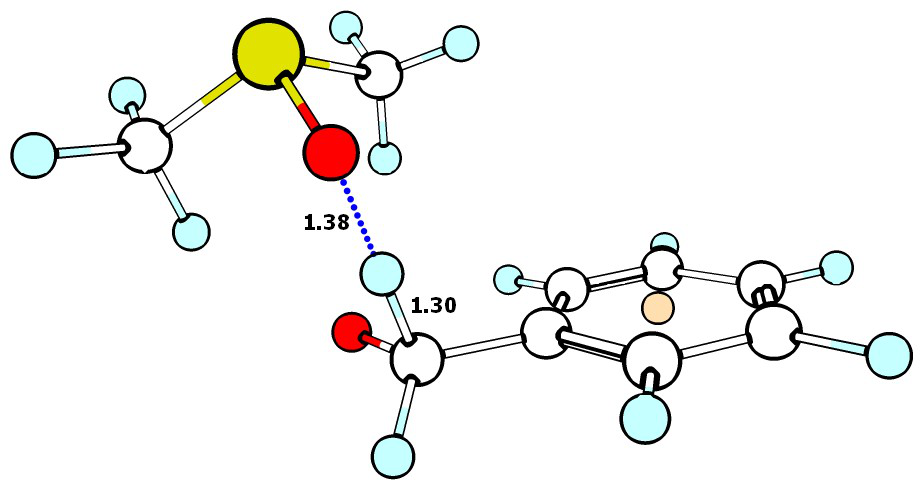
\includegraphics[width=4cm]{figures/dmso-bno-rev}
  }
  \subfigure[Alternative DMSO-NaCl + \bno]{
    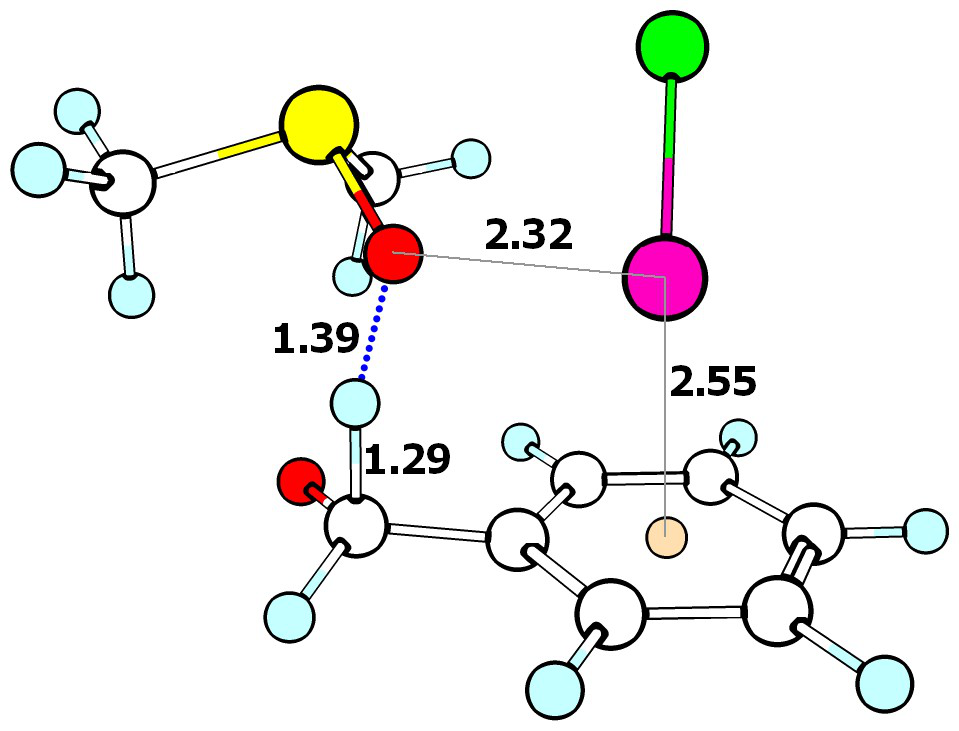
\includegraphics[width=4cm]{figures/dmso-nacl-bno-rev}
  }

  \subfigure[Conventional DMSO + \bno]{
    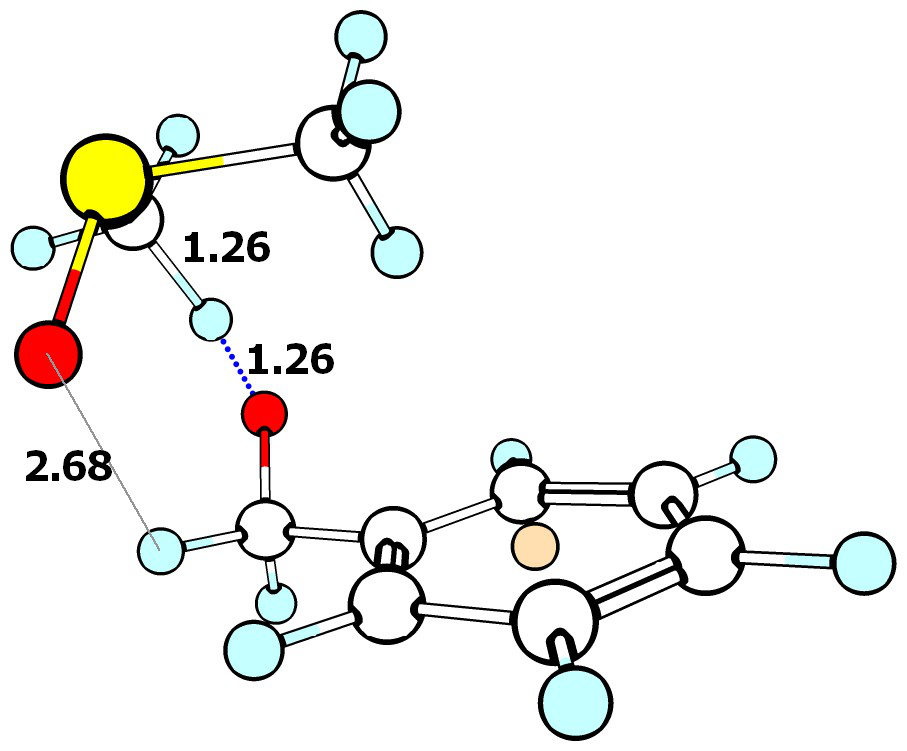
\includegraphics[width=4cm]{figures/dmso-bno}
  }
  \subfigure[Conventional DMSO-NaCl + \bno]{
    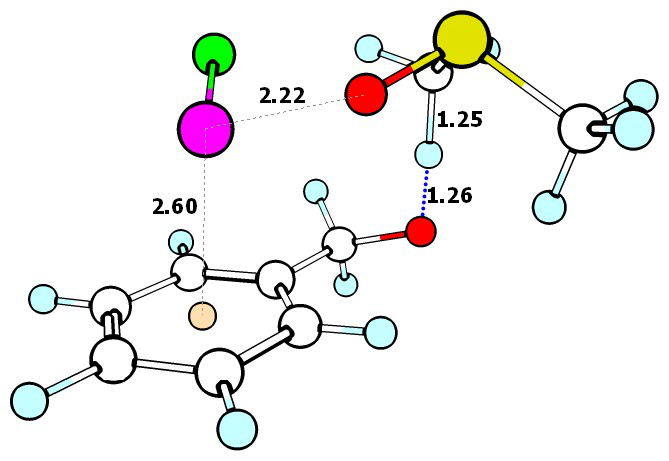
\includegraphics[width=4cm]{figures/dmso-nacl-bno}
  }

  \caption[TS structures of HAT reaction between DMSO and \cumo, and the
  reverse and conventional HAT reaction with \bno\ excluding and including
  \ch{NaCl}.]{TS structures of HAT reaction between DMSO and \cumo, and the
  reverse and conventional HAT reaction with \bno\ excluding and including
  \ch{NaCl}. Key interatomic distances are shown in units of \AA. Element
  colour key: white is carbon, light blue is hydrogen, red is oxygen, yellow is
  sulphur, purple is sodium, green is chlorine, and peach is a dummy atom in
  the centre of an aromatic ring.} \label{fig:dmso-ts}
\end{figure}

Focussing first of the reactions of DMSO with \cumo\ and \bno\ in the presence
of \ch{NaCl}. The reactions studied are shown in~\ref{fig:dmso-rxn} and the
calculated free energy (enthalpic) barriers are listed in~\ref{tab:dmso-dG}.
Also, the TS structures for the reactions in~\ref{fig:dmso-rxn} are shown
in~\ref{fig:dmso-ts}a-f. Firstly, for HAT between DMSO and \cumo\ in the
presence of \ch{NaCl} (Reaction 1,~\ref{fig:dmso-ts}b), the free energy barrier
increases by 1.5 \kcalmol\, however the enthalpic barrier decreases by 3.7
\kcalmol. This can be explained in a similar manner to the reactions of DMA:
\ch{Na^+} interacts both with the oxygen of DMSO and the aromatic system of
\cumo, resulting in a stabilization of the TS and a decrease in enthalpic
barrier in spite of a predicted increase in \ch{C-H} BDE. This binding however
results in a tighter TS structure, thus the entropic cost increases and so does
the $\Delta G^\ddagger$.

Next, the reaction of DMSO with \bno\ was previously
characterized\cite{Salamone2012} as occurring through the rate determining
formation of a strong pre-reaction complex, however, we recently showed the
reaction likely takes place through a reaction in which \bno\ acts as a
hydrogen atom donor, rather than acceptor.\cite{vanSanten2016} For this
alternative HAT between DMSO and \bno\ in the presence of \ch{NaCl} (Reaction
2,~\ref{fig:dmso-ts}d) the free energy barrier increases as a result of
complexation. This is appears to be an entropic effect as a result of binding,
as $\Delta H^\ddagger$ decreases by 1.2 \kcalmol\ due to the interaction of
\ch{Na^+} with DMSO and the aromatic ring of \bno. In this TS structure
excluding \ch{NaCl} there is some charge separation, however, DMSO (the
acceptor) has a partial positive charge and \bno\ (the donor) has a partial
negative charge. This is contrary to typical HAT reactions between
oxygen-centred radicals and \ch{C-H} bonds where in the TS structure, the donor
typically has a partial positive charge and the acceptor has a partial positive
charge. Therefore, the significant reduction in charge separation from 0.25
$e^-$ to 0.11 $e^-$ appears to play a lesser role. This may be due to the
non-Lewis electronic structure of sulfoxide compounds. The alternative HAT
reaction is likely driven by the concerted cleavage of the \ch{S=O} bond of
DMSO-H.

While the conventional HAT reaction between DMSO and \bno\ is unlikely to occur
as the barrier is ca. 12 \kcalmol higher than the alternative reaction, it is
still interesting to consider the effect that \ch{NaCl} has on the reaction
barrier height. \ref{fig:dmso-ts}f shows that in the TS structure for the
conventional HAT reaction between DMSO and \bno\ in the presence of \ch{NaCl},
there is a relatively close interaction with both the oxygen of DMSO and the
aromatic ring of \bno. As a result, the free energy (enthalpic) barrier
decreases by 0.6(5.2) \kcalmol. NPA estimates a relatively large (as compared
to the DMA HAT reactions) 0.10 $e^-$ charge transfer from DMSO to \ch{Na^+},
resulting in a decrease in charge separation in the TS structure from 0.27
$e^-$ to 0.21 $e^-$.

Turning now to the reactions of \bno\ with the substrates HMPA and TBPO, which
are closely related phosphine oxide compounds which are commonly used as
organic solvents. These two substrates are also closely related to DMSO in that
they are strong hydrogen bond accepting substrates, and therefore may undergo a
reverse HAT reaction in which \bno\ donates an acidic $\alpha$-\ch{C-H}
hydrogen atom, rather than accepting in the conventional manner. The reaction
coordinate diagrams from HMPA with \bno\ and TBPO with \bno\ are shown
in~\ref{fig:hmpa-tbpo-bno}a and b, respectively. In the possible reverse HAT
reactions for both substrates the free energy barrier is lower than the
conventional HAT barrier by 6 \kcalmol\ for HMPA and 10 \kcalmol\ for TBPO.
However, in both cases the process is energetically uphill, and so is unlikely
to occur. For both the radical products HMPA-H and TBPO-H, the cleavage of the
\ch{P=O} bond results in an additional 20 \kcalmol energy cost owing to the
significantly greater strength of \ch{P=O} bonds as compared to \ch{S=O} bonds
(The BDEs are 86 \kcalmol\ in DMSO vs. 147 \kcalmol\ in
HMPA).\bibnote{Calculated using the ROCBS-QB3 method.} Therefore, reverse HAT
reactivity is likely driven by the cleavage of the \ch{S=O} bond in DMSO.

\begin{figure}[!htbp]
  \centering
  \subfigure[HMPA + \bno]{
		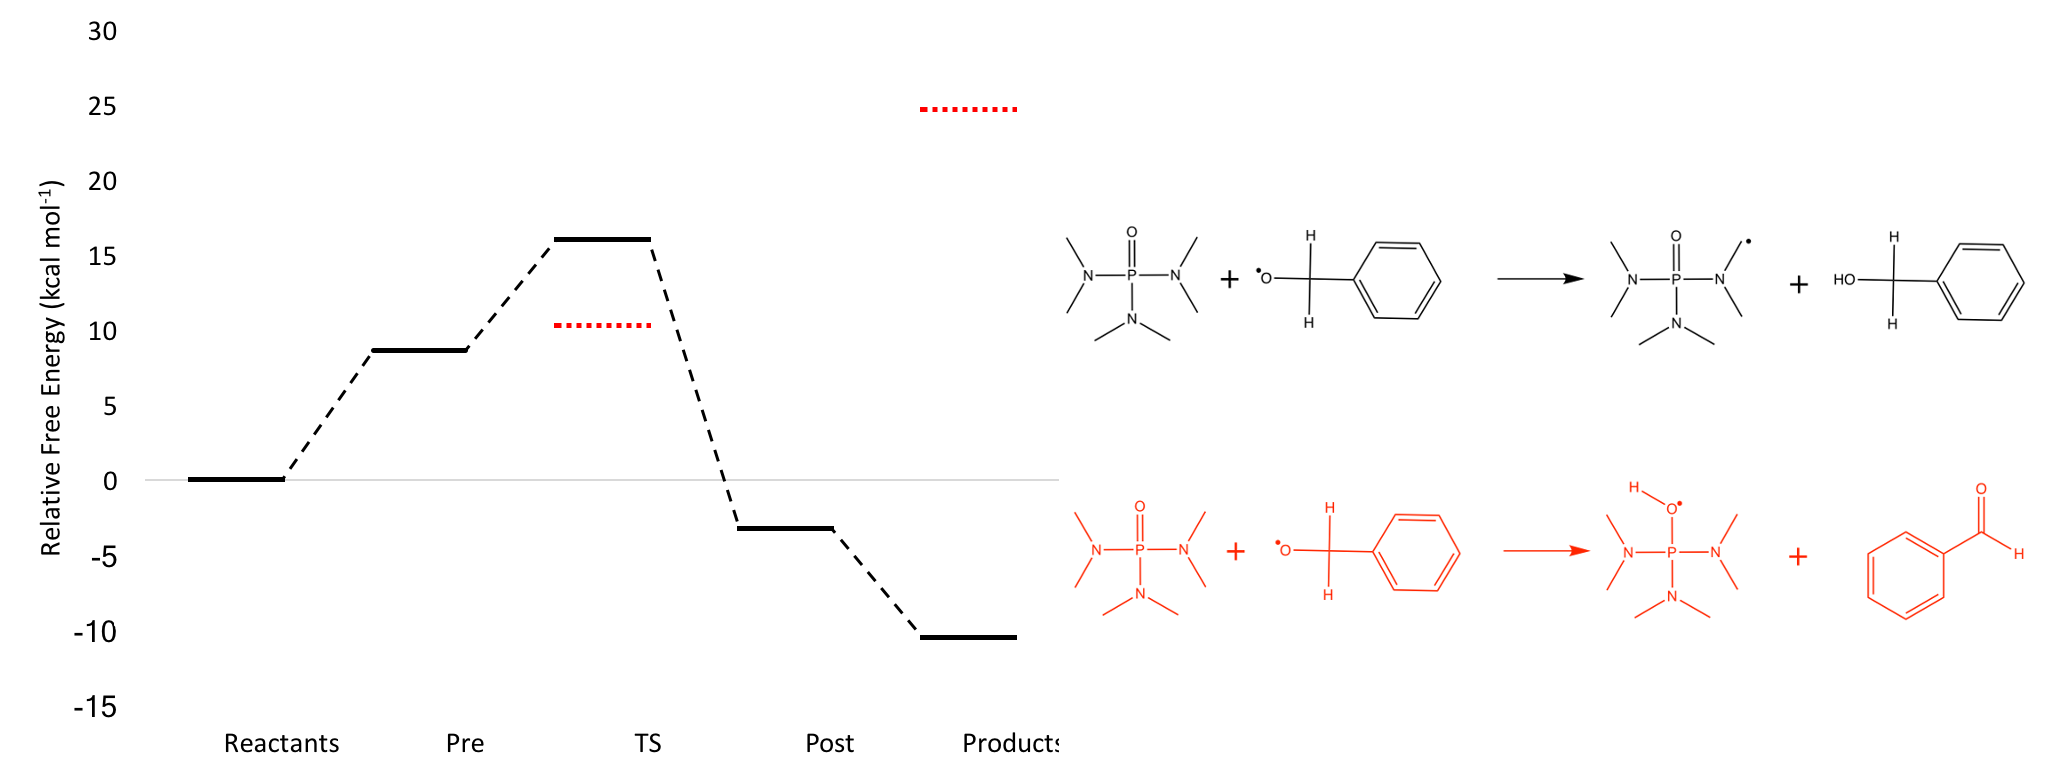
\includegraphics[width=12cm]{figures/hmpa-bno-rxn}
	}

  \subfigure[TBPO + \bno]{
		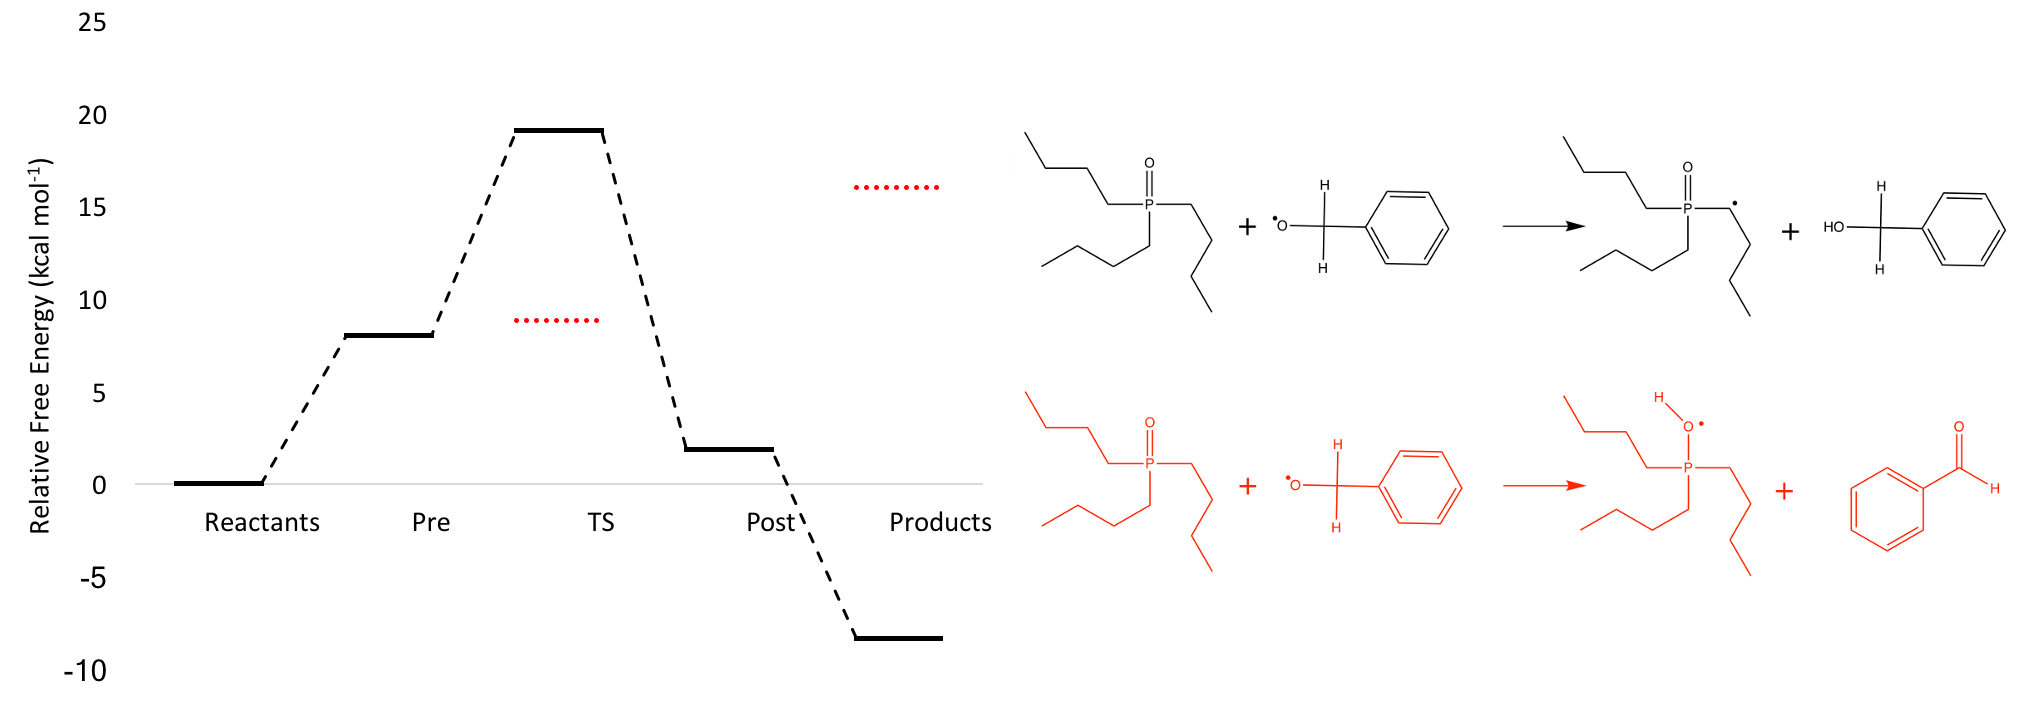
\includegraphics[width=12cm]{figures/tbpo-bno-rxn}
	}
  \caption[Reaction profiles for HAT between HMPA with \bno\, and TBPO with
  \bno.]{Reaction profiles for HAT between \textbf{a} HMPA with \bno\,
  \textbf{b} and TBPO with \bno. Relative free energies in \kcalmol\ are shown
  for the conventional (black) and reverse (red) HAT reactions.}
  \label{fig:hmpa-tbpo-bno}
\end{figure}


As HMPA and TBPO do not react via reverse HAT with \bno, I did not seek the
determine the effects of \ch{NaCl} on these reaction barriers. Note also, that
unlike DMSO, there is no strong hyperconjugative overlap between the \ch{S=O}
orbitals and the abstractable \ch{C-H} bonds of TBPO or HMPA. Therefore, the
effects of metal complexation to the phosphine oxygen (where \ch{Na^+} will
bind) should not significantly effect the \ch{C-H} bond strengths or enthalpic
barrier heights. The HAT reaction barrier heights of \ch{NaCl} with with HMPA
and TBPO for the HAT reaction with \cumo\ are listed in~\ref{tab:hmpa-tbpo}.
The TS structures for direct HAT reactions between HMPA or TBPO with \cumo\ and
\bno\ including \ch{NaCl} are shown in~\ref{fig:hmpa-tbpo-ts}.


\begin{table}[!htbp]
\caption[Calculated free energy (enthalpy) barrier for HAT between HMPA and
TBPO with \cumo\ with and without \ch{NaCl}.]{Calculated free energy (enthalpy)
barrier ($\Delta G(H)^\ddagger$, \kcalmol) for HAT between HMPA and TBPO with
\cumo\ with and without \ch{NaCl}. The change in barrier height is calculated
relative to the same reaction without the inclusion of \ch{NaCl}. All barrier
heights are relative to separated reactants and were calculated at the
M05-2X-SMD(MeCN)/6-311+G(2d,2p)//M05-2X/6-31+G$^{**}$ level of theory.
$^*$Indicates estimated barrier based on ``guess'' TS structure.}
\label{tab:hmpa-tbpo}
\begin{tabular}{l c c}
Reaction   &  $\Delta G(H)^\ddagger$ &  $\Delta \Delta G(H)^\ddagger$ \\
\hline
HMPA + \cumo      &  17.4(3.8)       &                            \\
HMPA-NaCl + \cumo &  12.8(-1.0)$^*$  &  -4.6(-4.8)                \\
HMPA + \bno      &  16.0(2.6)        &                            \\
HMPA-NaCl + \bno &  14.5(1.6)$^*$    &  -1.5(-1.0)                \\
TBPO + \cumo      &  20.1(6.8)       &                            \\
TBPO-NaCl + \cumo &  21.6(6.0)       &  1.5(-0.8)                 \\
TBPO + \bno      &   19.0(6.9)      &                            \\
TBPO-NaCl + \bno &   19.1(4.8)      &   0.1(-2.1)                \\
\end{tabular}
\end{table}

\begin{figure}[!htbp]
  \centering
  \subfigure[HMPA-NaCl + \cumo]{
		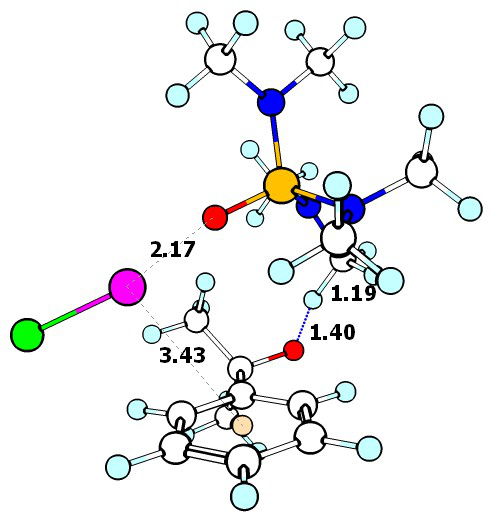
\includegraphics[width=4cm]{figures/hmpa-nacl-cumo}
	}
  \subfigure[HMPA-NaCl + \bno]{
		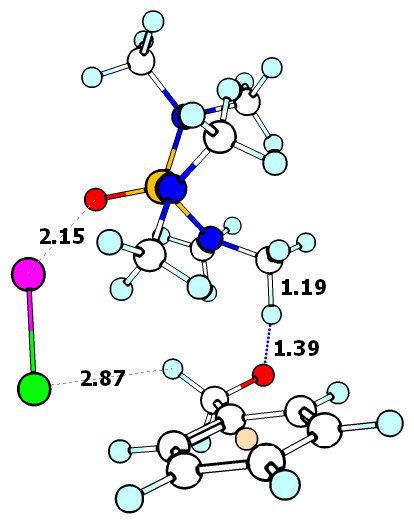
\includegraphics[width=4cm]{figures/hmpa-nacl-bno}
	}

  \subfigure[TBPO-NaCl + \cumo]{
    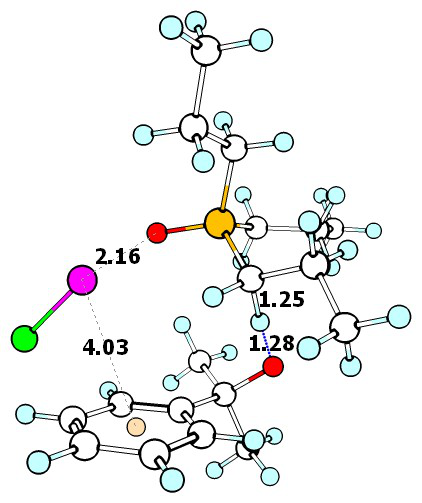
\includegraphics[width=4cm]{figures/tbpo-nacl-cumo}
  }
  \subfigure[TBPO-NaCl + \bno]{
    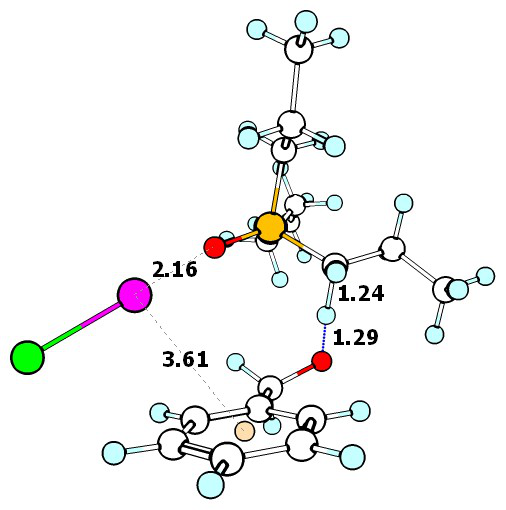
\includegraphics[width=4cm]{figures/tbpo-nacl-bno}
  }

  \caption[TS structures of HAT reaction between HMPA and TBPO with \cumo\ and
  \bno\ including \ch{NaCl}.]{TS structures of HAT reaction between HMPA and
  TBPO with \cumo\ and \bno\ including \ch{NaCl}. Key interatomic distances are
  shown in units of \AA. Element colour key: white is carbon, light blue is
  hydrogen, red is oxygen, orange is phosphorous, purple is sodium, green is
  chlorine, and peach is a dummy atom in the centre of an aromatic ring.}
  \label{fig:hmpa-tbpo-ts}
\end{figure}

For HMPA with \cumo\ and \bno\ in the presence of \ch{NaCl}, the HAT reaction
barrier decreases in both cases. For the reaction with \cumo\
(\ref{fig:hmpa-tbpo-ts}a), this can be explained on the basis of the
interaction between \ch{Na^+} with both the phosphine oxygen and the aromatic
system of \cumo. However for the reaction with \bno\ (\ref{fig:hmpa-tbpo-ts}b),
there is not such interaction with the aromatic system of \bno. In this case,
the decrease in reaction barrier can be ascribed to the lack of rotation of the
\ch{CH2O^.} moiety of \bno. In the HAT reaction between HMPA and \bno\
excluding \ch{NaCl}, there is a rotation of this moiety by ca. 30$^\circ$. The
complexation of \ch{NaCl} breaks the hydrogen bond between the
$\alpha$-\ch{C-H} bond of \bno\ with the oxygen of HMPA, and forms a now
interaction between \ch{Cl^-} and the $\alpha$-\ch{C-H} bond of \bno. This new
interaction stabilizes the TS and allows the oxygen-centre of \bno\ to remain
in the plain of the aromatic system.

Finally, for the reactions of TBPO with \cumo\ and \bno\ there are long range
interactions of \ch{Na^+} with the aromatic systems resulting in a decrease in
$\Delta H^\ddagger$. The free energy barrier for \cumo\ is not significantly
effected, while it increases by about 1.5 \kcalmol\ for \bno. This is likely
due to the longer range interaction of \ch{Na^+} with \cumo\ as compared to
\bno\ (4.0 \AA\ vs. 3.6 \AA, respectively).

\section{Summary}

The effects of non-redox active metal cations upon the barrier heights of HAT
reactions between small protein models and Lewis basic organic substrates with
oxygen-centred radicals were investigated herein. First, benchmark studies were
performed to determine the best available DFT-based method for studying the
interactions between alkali and alkaline earth metals with organic substrates
and radicals. Calculations of the gas-phase binding energies reveal that most
DFT-based methods can reasonably predict the binding interactions.

\jnote{I have decided not to write this until you (Gino) have had a chance to
review this chapter.}
